\documentclass{uvamscse}

\usepackage{todonotes}
\usepackage{verbatim}
\usepackage{graphicx}
\usepackage{array}
\usepackage{caption}

\usepackage[T1]{fontenc}
\usepackage{inconsolata}

\usepackage{listings}
\usepackage{color}



%Commands and Macros
\newtheorem{definition}{Definition}[section]

%\newenvironment{definition}[1][Definition]{\begin{trivlist} 
%\item[\hskip \labelsep {\bfseries #1}]}{\end{trivlist}}


% Author abbreviations
\newcommand{\toolName}{Skunk Debunk}

\newcommand{\Atestbugs}{Vahabzadeh et al.}
\newcommand{\AtestCodeQuality}{Athanasiou et al.}
\newcommand{\ACoEvolution}{Zaidman et al.}

\newcommand{\AFBEval}{Ayewah et al.}
\newcommand{\AFB}{Hovemeyer et al.}
\newcommand{\AComparisonBugTools}{Rutar et al.}

\newcommand{\Afixture}{Greiler et al.}
\newcommand{\Aobsolete}{Hao et al.}
\newcommand{\AfalseAlarms}{Herzig et al.}
\newcommand{\Aflaky}{Luo et al.}
\newcommand{\AclusterFailure}{DiGiuseppe et al.}

\newcommand{\AtestSmell}{Moonen and van Deursen}
\newcommand{\AtestDependence}{Zhang et al.}
\newcommand{\AtestFixture}{Greiler et al.}
\newcommand{\AtestxUnit}{Mezaros}

\newcommand{\AbayesianDetectCodeDesignSmells}{Khomh et al.}
\newcommand{\AsmellsEmpiric}{Bavota et al.}
\newcommand{\AdetectionStrategies}{Marinescu}
\newcommand{\AsigTS}{Van Rompaey et al.}

\newcommand{\Aframework}{Brand et al.}


\usepackage{listings}

\lstdefinelanguage{sdf}{%
  numbers=none,
  morekeywords={module,imports,exports,sorts,context,lexical,free,syntax,==,=,+,-,left,cons,prefer,avoid,bracket},
  columns=flexible,
  morestring=[b]",
  basicstyle=\footnotesize\mdseries,
  literate={->}{{\,\,$\to$\,\,}}1
}

\lstdefinelanguage{dcg}{%
  numbers=none,
  morekeywords={},
  morestring=[b]",
  basicstyle=\footnotesize\mdseries,
  columns=flexible,
}

\lstdefinelanguage{prolog},
  literate={:-}{{\,$\Leftarrow$\,\,}}1 {-->}{{$\to$\,}}1
}

\lstdefinestyle{mono}{
  basicstyle=\footnotesize\ttfamily
}

\lstset{%
  frame=none,
  xleftmargin=2pt,
  stepnumber=1,
  numbers=left,
  numbersep=7pt,
  numberstyle=\ttfamily\scriptsize\color[gray]{0.3},
  belowcaptionskip=\bigskipamount,
  captionpos=b,
%  escapeinside={*'}{'*},
  % language=fl,
  tabsize=2,
  emphstyle={\bf},
  stringstyle=\itshape,
  showspaces=false,
  keywordstyle=\bfseries\rmfamily,
  columns=flexible,
  basicstyle=\small\mdseries,
  showstringspaces=false,
}

\newcommand{\cmd}[1]{\texttt{$\backslash$#1}}

\title{Detecting Test Bugs Using Static Analysis Tools}
% \coverpic[100pt]{figures/terminal.png}
\subtitle{}
 \date{Q1 2016}
 
 
 

\author{Kevin van den Bekerom}
\supervisor{dr. Magiel Bruntink, \url{m.bruntink@sig.eu}}
\authemail{kvandenbekerom@sig.eu}
\host{Software Improvement Group, \url{https://www.sig.eu/}}

\definecolor{mygreen}{rgb}{0,0.6,0}
\definecolor{mygray}{rgb}{0.5,0.5,0.5}
\definecolor{mymauve}{rgb}{0.58,0,0.82}

\lstset{ %
	numbers=none,
	backgroundcolor=\color{white},   % choose the background color
	basicstyle=\footnotesize,        % size of fonts used for the code
	breaklines=true,                 % automatic line breaking only at whitespace
	captionpos=t,                    % sets the caption-position to bottom
	commentstyle=\color{mygreen},    % comment style
	escapeinside={\%*}{*)},          % if you want to add LaTeX within your code
	keywordstyle=\color{blue},       % keyword style
	stringstyle=\color{mymauve},     % string literal style
	 frame=lrb, rulesepcolor=\color{black},
	 rulecolor=\color{mygray},
	tabsize=4 % same as written code. 	
}

 \DeclareCaptionFont{blue}{\color{blue}} 
 
 \captionsetup[lstlisting]{singlelinecheck=false, labelfont={blue}, textfont={blue}}
 
 \DeclareCaptionFont{white}{\color{white}}
 \DeclareCaptionFormat{listing}{\colorbox[cmyk]{0.83, 0.35, 0.35,0.01}{\parbox{\textwidth}{\hspace{15pt}#1#2#3}}}
 \captionsetup[lstlisting]{format=listing,labelfont=white,textfont=white, singlelinecheck=false, margin=0pt,	
 	 font={bf,footnotesize}}

\begin{document}
\maketitle

%%%%%%%%%%%%%%%%%%%%%%%%%%%%%%%%%%%%%%%%%%%%%%%%%%%%%%%%%%%%%%%%%%%%%%%%%%%%%%%%
\chapter*{abstract}
\todo{write when test smell results are in}

\chapter{Introduction}
A software developer writes tests to assert correct behavior of the System Under Test (SUT). As with writing production code, software developers can make mistakes in writing test code. The errors that occur when a developer makes a mistake in writing test code are referred to as Test Bugs (TB). A TB is either a false positive test failure, or false negative test failure. The focus of this thesis is on False Positive test cases. A false positive test case fails whereas the production code was correct.

The topic of TBs has not received much attention. \Atestbugs{} conducted an empirical study of Test Bugs in 2015, categorizing TBs for the first time \cite{vahabzadeh2015empirical}.  

\section{Initial study}
As of 2015, no study existed that categorized bugs in test code. \Atestbugs{} researched many open source projects, written in different programming languages to find out what categories of test bugs existed in test code \cite{vahabzadeh2015empirical}. A test bug is either a False Positive (test fails but no defect in production code), or Silent Horror (test passes, but should have detected a bug in production code). 

\Atestbugs{} started looking for issues in Issue Tracking Systems (in particular JIRA). If these issues were later resolved, with a fix in test code, they classified the issue as a test bug. From the set of test bugs they obtained (5556) they sampled 443 cases which have undergone manual inspection. They categorized each TB in the sample, resulting into 6 broad categories and 16 subcategories. Table \ref{table:TBcategories} provides an overview of the percentages. Each category is explained in Chapter \ref{ch:background}. For false positives, the most prominent categories were semantic bugs and flaky tests. Silent horror tests (test passes although there is a bug in production code) contribute to only 3\% of all test bugs.

\begin{table}[]
	\centering
	
	\label{my-label}
	\begin{tabular}{ll}
		\textbf{Category} & \textbf{Percentage of TBs}  \\
		\hline
		Semantic          & 25                         \\
		Flaky             & 21                         \\
		Resource          & 14                         \\
		Environment       & 18                         \\
		Obsolete          & 14                         \\
		Other             & 8                         
	\end{tabular}
	\caption{Test Bug prevalence per category}
\end{table} 

\Atestbugs{} also researched the issue solving differences between test code and production code bugs. They found that test bugs were solved much faster than production code bugs. 

Finally they investigated whether popular bug solving tools could find test bugs they categorized. For FindBugs, they found that the tool could not find a single test bug.

\section{Problem statement}
\Atestbugs investigated what TBs FindBugs could find. Their findings were that \emph{``Findbugs could not find any of the test bugs in our sampled 50 bug reports''} \cite{vahabzadeh2015empirical}. Are static source code analysis tools that bad in finding TBs? How do other tools fare? And what about the small sample? Are their results generalizable? Has anything been done on detecting TBs since the introduction of their paper? 

In short there are enough reasons to replicate the Findbugs study of \Atestbugs{} Consider that no tool can find TBs. What would be necessary to actually find TBs? 

One of the approaches is relating Test Smells to Test Bugs. A Test Smell is a pattern indicating bad test code, for a number of possible reasons. The test code can be unmaintainable, brittle or hard to read. Test Smells are measurable with static source code analysis techniques. The existence of a relation between test smells and TBs could be the basis for developing a tool to detect/prevent/predict TBs.

\subsection{Research questions}
The research questions are named after the Chapter in which they are answered. Our research is two-fold. For one, we assess the ability of SSCATs to detect TBs. Secondly, we explore options to improve the result of TB detection.

\subsubsection{TB detection by SSCATs}
\textbf{RQ3.1: What test bugs, as described by \Atestbugs{} can popular Java bug finding tools \footnote{FindBugs, PMD, JLint, SonarQube} find?} \label{RQ_3.1} \\

Is there a difference among SSCATs in what TBs they can find? Do we get the same findings as \Atestbugs{}?\\ \\
\textbf{RQ3.2: To what extent can static source code analysis techniques be used to find test bugs?} \\
\label{RQ_3.2}

What is different about TBs, as compared to production code bugs that they are so hard to find? Can we make suggestions on how current SSCATs can extend their analysis to find more TBs?

\subsubsection{Improve TB detection by measuring Test Smells}
\textbf{RQ4.1: Does bad test code indicate test bugs? \label{RQ_4.1}} \\

We will answer this question by looking at the test smells occurring in the code affected by the test bug. We want to see if there are significantly more, or worse test smells as compared to``bug free'' parts of the system.\\ \\
\textbf{RQ4.2: Can we use test smells to predict the occurrence of test bugs?} \\
\label{RQ_4.2}

For each test smell we can measure its severity. Do test bugs occur in parts of the system that have test smells of high severity? Are there healthy parts of the system that  also contain test smells of high severity?

\subsection{Solution outline}
To assess the ability of SSCATs to find TBs, we will look at the difference in reported issues between two consecutive commits. One of which is the commit that solved the TB. If a difference is reported, we still need to know
if the reported issues point to the TB. All used rules in SQ are mapped to categories of TBs they could find. So when an issue appears in the \texttt{diff}, points to the correct location, and is mapped to the correct category, we speak of a True Positive, i.e. the SSCAT could find the TB.

Doing the analysis constitutes of:
\begin{enumerate}
	\item Checkout issue-solving commit and run SQ. Afterwards collect the issues set $A$.
	\item Checkout commit just before the issue-solving commit and run SQ. Afterwards collect the issues set $B$.
	\item Compute the difference: $B\setminus A$, i.e. all issues that disappeared when resolving the TB.
	\item Manually check the difference on points described above.
\end{enumerate}

To answer research questions RQ4.1 and RQ4.2 (\ref{RQ_4.1}), we will build a tool that detects test smells with static source code analysis. We measure several systems by checking out the system just before the bug-fix, and running our tool on the system. We measure the severity of the parts of the source code affected by the TB. We relate this to the overall quality of the system, in terms of test smells.
\subsection{Research method}
In Chapter 3 we did a replication study of the FindBugs study done by \Atestbugs{} A replication study is conducted with three possible variables to change; dataset, subject under study, research method. We kept the research method the same, used the same dataset of TBs (ASF systems), but changed the subject of study (SonarQube instead of FindBugs). For the analysis we employed a mixed-methods approach. Quantitative analysis revealed the TB-finding capabilities of SonarQube. Qualitative analysis of the results provided insights into why certain TBs could not be found.

\todo{Second study Chapter 4}
\section{Contributions}
\begin{enumerate}
	\item The concept of \emph{test bug} is explained. Several (real-world) examples are given, for a large number of different categories.
	\item SonarQube, a static source code analysis tool, is assessed on its ability to find TBs. SonarQube has a couple rules that can detect TBs in special cases, but this is for a marginal set of all TBs. 
	\item The corrolation between a diverse set of Test Smells and Test Bugs is investigated.
	\item A tool; \toolName, that finds Test Smells based on static source code analysis.
\end{enumerate}

\section{Related work}
\subsection{Detecting TBs}
\Aobsolete{} adopted the Best-First Decision Tree algorithm to classify regression test failures as coming from production or test code \cite{hao2013bug}. Seven features of tests (static and light-weight dynamic ) are identified to train a classifier.  
 
Their study was performed on two medium-size Java systems. Three studies were conducted: training set in same version as test set, in different versions, or in different programs. For the same-version experiment the machine learning classification method produced 80\% accuracy. For different versions the accuracy was even higher, around 90\%. Different programs resulted in decreased accuracy (around 60\%). 50\% is considered guessing. \\

Herzig et al. \cite{herzig2015empirically} tried to reduce the number of false alarms in test bugs during integration testing. They used associate learning to classify issues about test bugs being false positives. Accuracy was about 85-90\% with the number of correctly detected false positives at the end ranged from 34 to 48\%. They mainly investigated integration tests on two Windows systems for a period between one and two years. \\

\AtestDependence{} studied test dependence. A test $tA$ depends on $tB$ if the outcome of running $tA$ after $tB$ differs from reversing the run order. Based on the investigation of 5 real-world subject programs they concluded that in most cases (82\%) it takes at most two tests to manifest the dependent behavior \cite{zhang2014empirically}. \AtestDependence{} implemented four different algorithms to detect test dependencies. \\
\\
\textbf{Reverse-order}\\
Given a test-suite, the reverse-order algorithm executes each test in the normal order obtaining the expected result. Then the tests in the test-suite are executed in reverse-order. Any test that exhibits a different result is possibly dependent.\\
\\
\textbf{Randomized}\\
Same approach as reverse-order, but randomizes the execution order, which is done $n$ times. This algorithm proves the most efficient to find a reasonable amount of test dependencies. Which test depends on which test still has to be determined by the user. \\
\\
\textbf{Exhaustive bounded}\\
Executes all ordering-permutations of $k$ tests for a given test-suite. This analysis technique is more time-consuming but gives sets of dependent test cases (usually pairs, or singles). \\
\\
\textbf{Dependence-aware bounded}\\
Exhaustive-bounded examines all $k$ length permutations of a test-suite. Dependence-aware algorithm clusters tests by the fields they read and write. It runs once for $k = 1$ identifying all tests that do not access global variables or resources, excluding them from the search set. The results from Dependence-aware bounded are the same as exhaustive-bounded, but requires less time to run. However, this analysis technique requires tracking the read and write operations of tests.  

\subsection{Production and Test Code evolution}
\ACoEvolution{} mined software repositories to study the co-evolution of production and test code \cite{zaidman2008mining}. They visualized the different views (co-evolution patterns) using a dot chart with colors.

The change history view plots addition and modification of unit tests, and units under test. Unit tests and units under test are plotted on the same horizontal line. Each vertical represents a commit. A vertical bar of the same color can represent work on a lot of test cases. 

The growth history view plots several size metrics (production lines of code, test lines of code, number of classes, etc.) of production and test code against each other to reveal growth patterns. \ACoEvolution{} use an arrow grid to summarize the different growth behaviors. 

The test quality evolution view plots test code coverage against test code volume for minor and major releases. An increasing line in coverage represents good test health. 

\ACoEvolution{} applied their model on two Java programs: Checkstyle and ArgoUML. They found periods of pure test code writing. They also found simultaneous introduction of test and production code. For Checkstyle, size metrics of test and production code followed each other closely. For ArgoUML, they witnessed a more staged approach, i.e. periods of low increase in test code size, followed by periods of high increase in test code size. No system showed a sharp increase in testing effort just before a major release. Test-Driven Development could be detected for Checkstyle. The also found that test code coverage grows alongside test code fraction. 

\subsection{(Test) Code Smells}
Marinescu \cite{marinescu2004detection} proposed a way to systematically detect design flaws using a number and composition of metric-based rules. The purpose of his work was to detect the ‘disease’ instead of symptoms (metrics), which could potentially point to a software disease, but require an analyst to draw conclusions. 

The detection strategy consists roughly of two steps. Step 1 is data filtering, where the detection strategy defines whether to use relative, absolute, statistical or interval filtering. Step 2 is a composition of data filters using Boolean logic and set operators. This results in a set of candidates potentially affected by the design flaw. 

Marinescu used his method to design detection strategies for 9 well-known design flaws and validated the approach on one open source system with two different versions.  Average accuracy was 67\%, where 50\% defines guessing.\\

Bavota et al. \cite{bavota2012empirical} talk about the diffusion of test smells among test classes. There is an high percentage of test classes having at least one test smell. Test smells are categorized by hand, based on the list of van Deursen. The correlation between test smells and several metrics \textit{(LOC, \#testclasses, \#testmethods, \#tLOC, ProjectAge, testCodeAge, teamSize) }reveals importance of test smells. Some smells are more prevalent as others. Assertion roulette, which occurs when a method has multiple assertions and at least one without explanation , is the most occurring (55\%). Eager test, which uses more than one method from the tested class comes second (34\%). 

They also studied the effect of test smells on maintenance. They held a questionnaire among different groups of students and software engineers. Among groups, experience level was roughly the same. Between groups, experience level varied. Bavota et al.  measured correctness in answering questions about tests with and without test smells. For each question, the time to answer that question was measured as well. 

The eager test smell has a strong significant negative correlation with precision. Test subjects were more precise in answering questions about the refactored test method as opposed to the method still containing the eager test smell. The eager test smell is the only smell that showed a significant strong correlation between time. Test subjects took more time when answering the question with the test smell as opposed to without.

Their main conclusions were that test smells generally have a negative impact on correctness. No significant impact on time was found. Experienced developers experience negative impact on correctness with only 3 test smells, as opposed to first year bachelor students. This group experienced difficulty with at least 6 test smells.\\


\Afixture{} extended the Test Fixture test smell, as presented by van Deursen \cite{van2001refactoring} into five additional Test Fixture smells \cite{greiler2013automated}. A test fixture is a way to setup a (unit) test, e.g. bringing the system into the correct state, accessing resources, etc. An \textit{inline-setup} occurs when a test method has all the setup code inside the method. Helper methods can also contain the setup code, which is called \textit{delegate} setup. When features of the jUnit framework (naming conventions, annotations) are used to mark setup methods, it is called \textit{implicit setup}. Test Fixtures are:

\begin{itemize}
	\item \textit{General Fixture}: Broad functionality in implicit setup and tests only use part of that functionality.
	\item\textit{ Test Maverick}: Test class contains implicit setup, but test case in class is completely independent of that setup.
	\item \textit{Dead Fields:} Test class or its super classes have fields that are never used by any method in the test class.
	\item \textit{Lack of Cohesion of Test Methods}: Test methods grouped into one class are not cohesive.
	\item \textit{Obscure-In-Line-Setup:} Covers too much setup functionality in the test class.
	\item \textit{Vague Header Setup:} Fields are initialized in the header of the test class but never used in the implicit setup.
\end{itemize}

Fixture usage is analyzed by using static code metrics. After invention of code metrics they mapped them to fixture strategies. For some, certain thresholds had to be set. The analysis was done in 3 steps; Fact extraction (metrics), analysis (using metrics, mapping to fixture strategies) and presentation. \Afixture{} found that fixture related test smells occur in practice, where 5 to 30 \% of the methods / classes are involved. Developers recognize the importance of high test code quality and that reduction in test code quality can lead to maintenance problems. They sometimes introduce fixture smells on purpose. \\

Khomh et al. implemented a detection method using Bayesian Belief Networks (BBN)\cite{khomh2009bayesian}. A BBN assigns probabilities to classes having a code smell. This allows analysts and developers to prioritize issues, which is not possible using the Boolean approach of classification. 

Khomh et al. trained a BBN with data from two medium sized open source Java projects. They illustrated their approach on the Blob (God Class) anti-pattern. First they instructed undergraduate and graduate students to identify all Blob classes in the Java programs under study. They constructed a BBN using rules established by previous research (Moha et al. \cite{moha2010domain}). The BBN was then trained by using information about the number of identified Blob classes in both programs. 

Khomh et al. showed that a BBN can be used to prioritize design issues by giving probability to classes potentially having a design smell. Their method was evaluated against the DECOR method from Moha et al.\cite{moha2010domain} The BBN approach showed better results (accuracy and recall). Accuracy was around 60 \%, where recall of 100 \% was achieved. The BBN can also be calibrated for a specific context (e.g. adjusting the impact of rules) to increase its accuracy even further. \\



\section{Outline}


\chapter{To what extent can static source code analysis tools detect test bugs?}
\label{ch:SQ}
There exist many tools to find bugs in source code. They range from purely static source code analysis, to fully dynamic analysis. In between there is byte-code analysis, which requires compiled code. Since static source code analysis tools can find a wide range of production bugs, why can they not find any test bugs? At least, according to \Atestbugs{} they cannot. They investigated the bug-finding capability of FindBugs for Java, which resulted in zero test bugs being found\cite{vahabzadeh2015empirical}.  In this chapter we will replicate their study, improve some aspects of their experiment design, and show for another popular static source code analysis tool, SonarQube, which test bugs it can find. We will answer research questions RQ3.1 and RQ3.2, see Section \ref{RQ_3.1}.

\section{Background}
\label{sec:background}

\Atestbugs{} empirically studied the repositories of Apache Software Foundation (ASF) projects and identified 5556 TBs \cite{vahabzadeh2015empirical}. They manually categorized 443 instances into 6 broad, and 16 subcategories. 

\subsection{Semantic Test Bugs}
\label{sec:semanticTB}
Semantic TBs occur when there is a mismatch between production and test code, or a mismatch between specifications. There exist several subcategories among semantic TBs. For each a simplified example is presented.

\subsubsection{Assertion Fault}
Fault in assertion expression or arguments of a test case. Something is checked that should not be checked, or an assertion is missing. For ACCUMULO-3290 the test failed when \texttt{scan} was not running. However, the scan could have status \texttt{QUEUED} and run at a later point. Therefore the test could fail prematurely. The fix was ignoring scans that had no \texttt{RUNNING} status. 

\begin{lstlisting}[language=java, caption=Assertion fault (ACCUMULO-3290), label=Code_TB_assertion]
for (String scan : scans) {
assertTrue("Scan does not appear to be a 'RUNNING' scan: '" + scan + "'", scan.contains("RUNNING"));
// actual testing
}
\end{lstlisting}

\begin{lstlisting}[language=java, caption=Assertion fix (ACCUMULO-3290), label=Code_TB_assertion_fix]
for (String scan : scans) {
if (!scan.contains("RUNNING")) {
log.info("Ignoring scan because it doesn't contain 'RUNNING': " + scan);
continue;
}
// actual testing
}
\end{lstlisting}


\subsubsection{Wrong control flow}
Mistakes in control flow structures (\texttt{if, switch, for, while, ...}) cause the test to wrongly fail. These errors expose a mismatch between the SUT and test code, e.g. the SUT assumes certain resources are excluded from the test, but the developer has to enforce this in the test case.

\subsubsection{Incorrect Variable}
When asserting the wrong variable, we speak of a semantic TB in the Incorrect Variable category. As an example consider TB DERBY-6716. A simple copy-paste error resulted in not testing adequately that \texttt{p1} equals \texttt{p2}, since only \texttt{p1} implies \texttt{p2} is tested.

\begin{lstlisting}[language=java, caption=Asserting the wrong variable (DERBY-6716), label=Code_TB_WrongVariable]
// test for equivalence, bug due to typo in second assert.
public void assertEquivalentPermissions() {
assertTrue(p1.implies(p2));
assertTrue(p1.implies(p2));
}
\end{lstlisting}

\subsubsection{Deviation from test requirements and missing cases}
Examples include missing a step to excessive the SUT correctly (MYFACES-1625), and miss setting some required properties of the SUT (CLOUDSTACK-2542) \cite{vahabzadeh2015empirical}. 


\subsubsection{Exception Handling}
A test could fail due to an uncaught exception, which is not relevant for the succes of the test case. The test then fails but the SUT might be correct. As an example consider Code snippet \ref{Code_TB_Exception}. In this simple example we want to test whether a list contains no elements. When the list is \texttt{null} however, the test will fail, but clearly the list contained no elements. In this case the developer should have caught the \texttt{NullPointerException} and pass it upstream.

\begin{lstlisting}[language=java, caption=Exception TB, label=Code_TB_Exception]
// test if list l is empty. Fails when list l is null.
public void testListContainsNoElements(List l)  throws Exception {
assertTrue(l.isEmpty());
}
\end{lstlisting}

\subsubsection{Configuration}
a TB in this category wrongly sets or uses a configuration object or file. There might also be an error in the configuration object/file itself. 

\subsubsection{Test statement fault or missing statement}
There is an error in the one of the statements of the test which may cause error in the SUT, e.g. not setting up the SUT correctly. A missing statement may result in not setting some required properties of the SUT.

\subsection{Flaky Test Bugs}
\Aflaky{} empirically investigated tests failing randomly, called \emph{flaky} tests \cite{2014empirical}. Flaky tests are tests that fail intermittently, even for the same software version. Flaky tests cause a number of problems for developers: hard to reproduce, due to non-deterministic behavior. Second, developers can spent a significant amount of time to determine the cause of failure, only to find out it is due to the test failing intermittently. Lastly, flaky tests may hide real bugs which developers might miss if they start ignoring tests that fail often. 

Flaky tests are divided into three categories: async wait, concurrency, and test order dependency. 

\subsubsection{Async wait}
Async wait tests make an asynchronous call to a service, but do not wait on that service to become available. There is no order-enforcing mechanism in place. A test dependent on a service will therefore fail when the service is not yet available but the test starts using the service. This can happen intermittently. For an example see Code Snippet \ref{Code_TB_AsyncWait}. We test whether HTMLService correctly retrieves the webpage error when we pass a non-existing address. If the server is slow in responding, the test will fail. Note that HTMLService will spawn a new thread to fetch the contents of the webpage. 

\begin{lstlisting}[language=java, caption=Async wait TB, label=Code_TB_AsyncWait]
public void testHTMLErrorCode() {
// request the contents of a webpage as a String, or the errorcode.
String htmlResponse = HTMLService.requestWebPage("www.google.com/search/for/existence/of/life");

// wait for a response from the server
Thread.sleep(1000);

// webpage does not exist (404 error)
assertEquals("404", htmlResponse);
}
\end{lstlisting}

\subsubsection{Concurrency}
Concurrency issues arise when another thread interacts in a non-desirable way with the thread the test is running in. Concurrency issues are exclusive to async wait issues. Common causes are data races, atomicity violations and deadlocks. For a trivial example take a look at DERBY-2799. The derby project contains tests for deadlock. It starts up a number of threads, which all print ``Starting Thread'' to the console. When a thread finishes work it prints ``Done Thread''. A test checks if all threads are started before any finishes. It might happen however that a thread finishes work, before all threads are started, resulting in a failing test. It should therefore be enforced that all threads are started before given the ability to continue. This issue is solved in Code snippet \ref{Code_TB_Concurrency_fix}

\begin{lstlisting}[language=java, caption=concurrency TB, label=Code_TB_Concurrency]
public void runThread(Thread t) {
System.out.println("Starting Thread");
t.start();
// do work ...
System.out.println("Done Thread");
}
\end{lstlisting}

\begin{lstlisting}[language=java, caption=concurrency TB fix, label=Code_TB_Concurrency_fix]
int startCount;

public void runThread(Thread t) {
System.out.println("Starting Thread");
synchronized (syncObject) {
startCount++;
syncObject.notifyAll();
while (startCount < THREAD_COUNT) {
syncObject.wait();	
}
}

t.start();
// do work ...
System.out.println("Done Thread");
}
\end{lstlisting}

\subsubsection{Test order dependency}
A test falls in the \texttt{test order dependency} category when its result depends on the order in which the tests are executed. A test $TC$ in this category may pass when test $TA$ runs before it, but may fail when test $TB$ is executed before $TC$. \Aflaky{} made this category for flaky tests, while \Atestbugs{} did not \cite{vahabzadeh2015empirical, 2014empirical}. They instead defined the \emph{Race Condition} category, which simply is part of the concurrency category defined by \Aflaky{} A test dependency failure is however not exclusively related to misuse of resources (as suggested by \Atestbugs). For that reason it is mentioned here again. An example of a test dependency bug is given in Section \ref{sec:TB_resource}. 

\subsection{Environmental Test Bugs}
Tests are written and execute properly in one environment (e,g. Windows), but fail in another (e.g. Linux). Common operating system related errors are: 
\begin{enumerate}
	\item Differences in path conventions
	
	\begin{lstlisting}[language=java, caption=Path convention bug, label=Code_TB_OS_path]
	public void test() {
	String testObject = "text(\"" + f.getAbsolutePath() + "\", \"avrodata\")";
	assertEquals(testObject, b);
	}
	\end{lstlisting}
	
	This test fails, since Windows uses \textquotesingle \textbackslash \textquotesingle{}  as its seperator for file names, therefore file names need to be escaped. This did not happen due to using the \texttt{File} (\texttt{f}) API. 
	
	\item File system differences: 
	\item File permission differences are different on different platforms.
	\item Platform specific use of environment variables.
\end{enumerate}
Alternatively, environmental issues can arise due to differences in JDK versions or vendor issues.


\subsection{Resource Test Bugs}
\label{sec:TB_resource}
Testing often involves setting up, or using resources, e.g. mock objects, reading/writing to a database or file, etc. Inadequately handling resources can affect other tests, even making them fail when they are essentially correct. One example is reverting changes to a database in the test method body. When this test fails due to an assertion failure, exception or timeout, resources are not properly reverted and other tests dependent on these resources will fail. 61 \% of resource related test bugs are due to test dependencies \cite{vahabzadeh2015empirical}. \Atestbugs posed an illustrative example. In code snippet \ref{Code_TB_RH_dep1}, when the test fails or an exception occurs, resources are not properly reverted. This risk is mitigated in code snippet \ref{Code_TB_RH_dep2} where \texttt{test()} is side-effect free.
\begin{lstlisting}[language=java, caption=Setup and Teardown with side-effects, label=Code_TB_RH_dep1]
@Test
public void test() {
acquireResources();
assertEquals(a, b);
releaseResources();
}
\end{lstlisting}

\begin{lstlisting}[language=java, caption=Setup and Teardown without side-effects, label=Code_TB_RH_dep2]
@Before
public void setUp() {
acquireResources();
super.setUp();
}

@Test
public void test() {
assertEquals(a, b);
}

@After
public void tearDown() {
releaseResources();
super.tearDown();
}
\end{lstlisting}

Common failure patterns are cleaning up resources in the test body, not calling \texttt{super.teardDwn()} or \texttt{super.setUp()}

\subsection{Obsolete Test Bugs}
\label{sec:obsoleteTB}
Writing code is an iterative process. As new requirements come, code changes, and tests have to be adjusted to properly assert that changes did not break the code. It can occur that tests become obsolete due to a change in the production code, e.g. old code is tested. The test will report a failure while the production code might be correct. 

When a test becomes obsolete and a developer determined that the SUT is correct, the test is modified in either the steps required to execute the SUT (77\%), or the assertion itself(23\%) \cite{vahabzadeh2015empirical}. 

A real world example is MAPREDUCE-5421 where a change in another system (YARN) caused a test to fail. Consider the following code snippet:

\begin{lstlisting}[language=java, caption=Obsolete TB, label=Code_TB_Obsolete]
public void testGetInvalidJob() throws Exception {
RunningJob runJob = new JobClient(getJobConf()).getJob(JobID.forName("job_0_0"));
assertNull(runJob);
}
\end{lstlisting}

\texttt{RunningJob} is a class in YARN that returned \texttt{null} when given invalid input, which is exactly what \texttt{testGetInvalidJob()} asserts. However, a change in \texttt{RunningJob} resulted in an \texttt{IOException} being thrown, instead of returning \texttt{null}. The changed behavior resulted in a test failure since an \texttt{IOException} is thrown, where a test success should have been reported. Code snippet \ref{Code_TB_Obsolete_Fix} fixes the bug by catching and checking that the right exception is thrown.

\begin{lstlisting}[language=java, label=Code_TB_Obsolete_Fix, caption=Fix for obsolete TB]
public void testGetInvalidJob() throws Exception {
try {
RunningJob runJob = new JobClient(getJobConf()).getJob(JobID.forName("job_0_0"));
fail("Exception is expected to thrown ahead!");
} catch (Exception e) {
assertTrue(e instanceof IOException);
assertTrue(e.getMessage().contains("ApplicationNotFoundException"));
}
}
\end{lstlisting}

\section{Experiment Design}

\subsection{Data set}
To determine which TBs can be found by regular SSCATs, we need to examine every type of TB. In practise this is infeasible. We therefore use a dataset containing a large set of categorized TBs, i.e. the dataset produced by \Atestbugs{} \cite{data}. By using this dataset, we can select TBs from every category, and more accurately measure the tools performance in finding TBs.

From this dataset, containing 443 TBs, we selected bugs from Java projects, which contained the most TBs. This selection is both practical and logical; SonarQube requires a license to run c++ code, which we did not possess. Java is the industry standard programming language. While analyzing only Java project hurts generalizability, analyzing Java projects itself is already valuable. 

\subsection{SSCAT selection and rule selection}
SonarQube is a tool that combines several SSCATs together into one result, but itself has a large number of rules as well. These rules do not rely on compiled code. As a result, the rules from SonarQube can find less elaborate patterns (bugs) as FindBugs and Infer \todo{ref to benchmark thingy}. FindBugs was already examined by \Atestbugs{}, but for a very small dataset. In their sample, no TB could be identified by FindBugs. They  randomly took TBs for which no category was determined. It could very well be the case that they missed some categories (which could be detected by FindBugs). In their paper they mention that FindBugs has rules for some of the TBs they found \cite{vahabzadeh2015empirical}. 

\subsubsection{SonarQube background}
SonarQube is a static source code analysis tool. It parses non-compiled source code and builds an Abstract Syntax Tree (AST). On top of that SonarQube contains a semantical API. Information regarding method parameter types, method return type, annotation types, \emph{uses}-relations, etc can be used. SonarQube allows defining a rule set to use for analysis. These rules can include FindBugs, PMD, Checkstyle and SonarQube rules. For FindBugs, the compiled code is required, since it analyzes Java byte-code. SonarQube also has some rules that rely on byte-code. 

\subsubsection{SonarQube vs Infer and FindBugs}
Infer is a SSCAT that uses model-checking to \emph{infer} Null-pointer dereferences and resource leaks. While only a small subset of all bugs in code, Infer is very good in finding these two categories of bugs \todo{Wouter to the rescue}. The question remains if Infer can find Resource Leaks for TBs. This question can be answered by selecting known resource-leak TBs and applying the analysis described in Section \ref{sec:TBanalysis} using Infer. This is left as future work.

FindBugs uses byte-code analysis to detect bug-patterns in code. Byte-code analysis requires the binaries of source code, i.e. compiled code. 

Both FindBugs and Infer are very hard to use on large open-source projects in the context of this study since these projects are very hard to build. For the analysis to be successful we must analyze the code of two consecutive commits. We can therefore not rely on jar files available online, for these are unavailable for specific commits. Building old versions of large open-source projects is also troublesome. Either a lot of dependencies are missing and cannot be downloaded online (address has been moved) or rely on an old execution environment (e.g. JVM). We therefore chose SonarQube to study a large set of TBs, albeit with less accurate analysis techniques. The development team of SonarQube have also been implementing a lot of FindBugs rules in the engine of SonarQube, such that one can simply select the SonarQube rule instead of using FindBugs.

\subsubsection{Rule selection}
A selection of rules is necessary to prevent getting overflowed with useless results. \Atestbugs{} simply selected all correctness and multi threaded correctness rules for FindBugs \cite{vahabzadeh2015empirical}. In the end they only looked at the difference in issues between two consecutive commits. Since we know more about TBs we can make a more guided selection of rules. Some TBs take multiple commits to solve, so the difference can potentially become much bigger. If we would select all SQ rules, these cases become unmanageable to investigate.

The candidate rules are selected based on expert opinion, by browsing the rules database of SonarQube, and searching for testing keywords, and keywords based on the categories defined by \Atestbugs{} \cite{vahabzadeh2015empirical}, e.g. \emph{flaky, resource, dependence, dependency, assertion}. 

\subsection{Analysis}
\label{sec:TBanalysis}
The analysis is automated as much as possible, to process a large amount of TBs, i.e. having processed sufficient TBs in each category. Figure \ref{fig:analysisFlow} gives a high level overview of the analysis process. We start by filtering the dataset (identified TBs) on programming language and project. Only the top 10 Apache projects are taken into account, for they contain more than 50\% of the identified test bugs (for Java). For all candidates (JIRA issue IDs) we check if it is possible to find the commit that solved the JIRA issue, since we need to check out the commit that solved the issue. We restrict the search to the master branch of each project. Some TB fixes are spread over multiple commits. In that case we consider the commit just before the first commit that provided a patch, and the commit that finally solved the TB. This process is illustrates in Figure \ref{fig:findCommit}. Commit $a$ is the commit just before the commit supplying the first Patch. In situation 1, the commit supplying the path is also the final commit. In situation 2, there are multiple patches ($b_1 .. b_n$), so $a$ remains the same, but $b$ becomes the final patch that fixed the TB ($b_n$).

\begin{figure}[!ht]
	\centering
	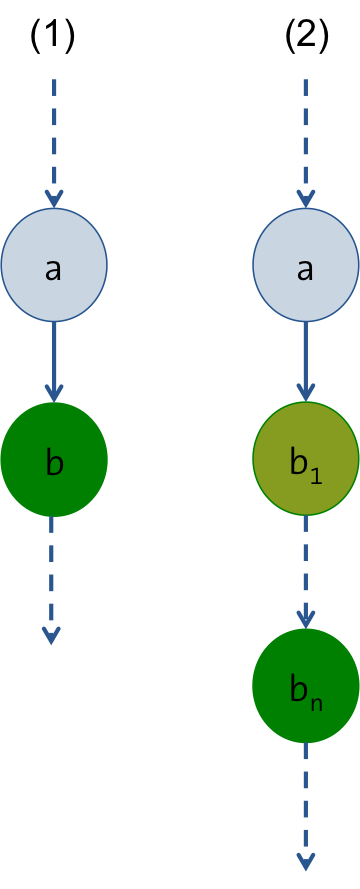
\includegraphics[width=0.2\textwidth]{figures/findCommit.png}
	\caption{Different scenarios when determining what commit to check out.}
	\label{fig:findCommit}
\end{figure}

After the pre-processing stage we have a set of TBs to analyze ($Analysis jobs$, see Figure \ref{fig:analysisFlow}). For the analysis we use the technique proposed by \Atestbugs{}, i.e. they ran a SSCAT on two consecutive commits and computed the difference in issues found \cite{vahabzadeh2015empirical}. Non-empty difference means that the patch took away issues, present in the previous version. The automation script checks out commit $a$ (see Figure \ref{fig:findCommit}) of the system under study on the SonarQube server, feeds that into the scanner, after which commit $b$ is checked out and analyzed. SonarQube does not provide rule location on method level (only exact source location), so we rely on SonarQube to compute the difference. The results of commit $a$ are downloaded from the server, as well as the difference, by using the SonarQube API. We store the issue set of snapshot $a$ for future analysis, see Section \ref{sec:TBresults} 

\begin{figure}[!ht]
	
	\centering
	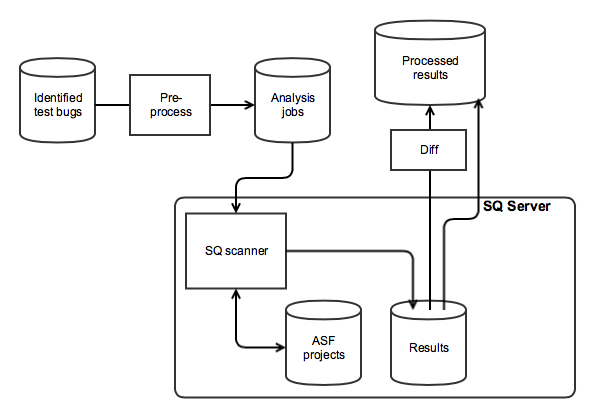
\includegraphics[width=0.8\textwidth]{figures/sqanalysisflowchart.png}
	\caption{Automated analysis steps}
	\label{fig:analysisFlow}
\end{figure}

All TB cases containing zero issues in the \emph{Diff}, see Figure \ref{fig:analysisFlow}, are  False Negatives (FN), i.e. SonarQube could not find the TB. The remaining cases are manually investigated. For each case we determine if it is a False Positive (FP) or True Positive (TP). To do this we drill down the data, answering questions in the following order: 

\begin{enumerate}
	
	\item Do issues reported by SonarQube appear at the correct location? SonarQube report the file in which the issue appears, and its source location. We check if these correspond to the locations of modified code by the patch. This does not have to be a one-to-one mapping. A bug fix can also improve some parts of the code, or modify parts due to dependencies upon the parts causing the TB.
	\item Do issues in the \emph{Diff} map to the correct TB category? Each rule we use is first mapped to one or more categories of TBs that it could possibly find. Finding an Exception issue in a flaky TB case is a FP for instance.
	\item If the issue appears at the correct location and is of the correct type, we still have to determine if it is pointed at the TB. Each TB is specific, irrespective of its category. The final step is based on expert opinion with the following question in mind: \emph{Could this issue have helped a developer find and fix the TB?}
\end{enumerate}


\section{Results}
\label{sec:TBresults}
\todo{No exception TBs in results, but say something about it, e.g. catching these with Exception rule in 2 out of ... times.}

First we give the overall results for SonarQube, which can be found in Figure \ref{fig:SQresults}. FN denotes that there was no difference in the amount of reported issues between two consecutive commits. The Patch that fixed the TB did not change the source code in a way such that issues disappeared. FP denotes the case were the difference contained more than one issue, but none of these were related to the bug category, or in a part of the code that could give developers an indication of the test bug being there. TP denotes the cases similar to a FP, but (a subset of) issues in the difference correctly indicated the occurrence of the TB. Some cases, labeled as UNKNOWN could not be resolved, usually because of the difference in issues between consecutive commits being unavailable. In these cases SonarQube could not resolve which issues changed, or the changed issues made no sense (changed set of issues being larger as the set of issues before the Patch).

\todo{Table with high level stats for investigated systems}
In total we examined 123 TBs, spread over 7 medium to large open source systems. An overview of the findings can be found in Figure \ref{fig:SQresults}. Of these, 94 (79\%) were False Negatives, 15 (13\%) False Positives, 7 (6\%) UNKNOWN, and only 3 (2.4\%) True Positives. All test bugs that could be found belonged to the Resource category, and were Operating System (OS) related. The JIRAID of the issues that could be found were: DERBY-576, DERBY-658 and DERBY-903. 

For DERBY-658 for instance, the issue was that the use of \texttt{String(byte[])} and \texttt{String(byte[], int, int)} constructors led to non-portable behavior. SonarQube has a rule (squid:s1943) to detect usages of these kind of functions. The difference for this case was 52 issues, of which 49 were squid:s1943. 

For the other two cases (DERBY-576, DERBY-903), the bugs were of a similar nature, and all reported issues in the difference set were squid:s1943.   

\begin{figure}[!ht]
	\centering
	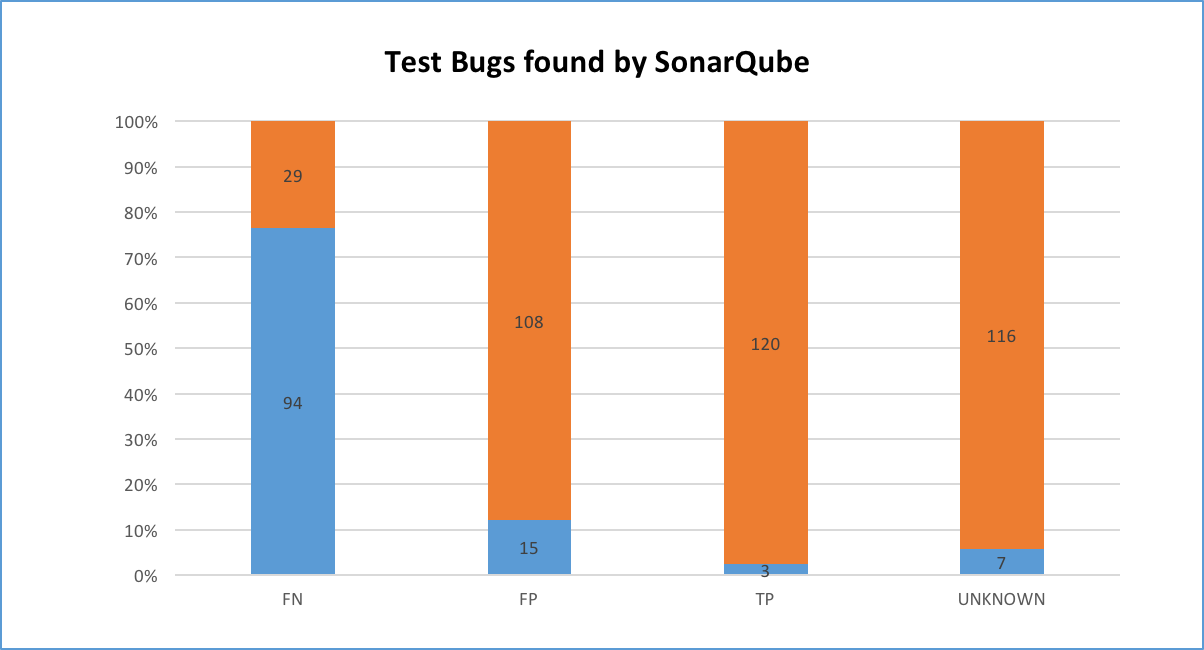
\includegraphics[width=0.7\textwidth]{figures/SQresults.png}
	\caption{FP, FN, TP and unknown rates}
	\label{fig:SQresults}
\end{figure}

We only investigated TBs of which the category has already been determined. Table \ref{table:sumCatTBs} shows how many TBs of each category were covered. This is a strict improvement over the work done by \Atestbugs, for they investigated TBs taken at random. We also investigated at least one TB for each of the subcategories defined by \Atestbugs, as described in Chapter  \ref{ch:background}.

\begin{table}[]
	\centering
	
	\label{table:sumCatTBs}
	\begin{tabular}{l|l}
		\textbf{Category}    & \textbf{Amount} \\
		\hline
		Semantic    & 24     \\
		Flaky       & 27     \\
		Resource    & 22     \\
		Environment & 16     \\
		Obsolete    & 20     \\
		Other       & 14    
	\end{tabular}
	\caption{Investigated test bugs per category}
\end{table}

For all the FP cases, we counted for each rule the number of times it appeared in the analysis. For each TB, a rule can appear once (meaning we did not count the total amount of results for each rule). Figure \ref{fig:SQRulesForFP} shows the results. Two of the FP cases are left out of the result, since they contained too many ($> 1000$) issues. Both had bugs caused by issues in non-java files (shell script and python files). A short explanation of what each rule detects can be found in Table \ref{table:SQrules}.

The first thing to notice is the low amount of different issues being present. In total we selected 35 SonarQube rules, of which only 11 appear in a difference set. We selected the rules that could find or indicate TBs. It is therefore surprising that such a small set of issues can be found. The issues that appear in Figure \ref{fig:SQRulesForFP} are also very general, e.g. s00112 (3 occurrences) and s2221 (4 occurrences) are general exception rules. \todo{if table is ready do more explanation}

\begin{figure}[!ht]
	\centering
	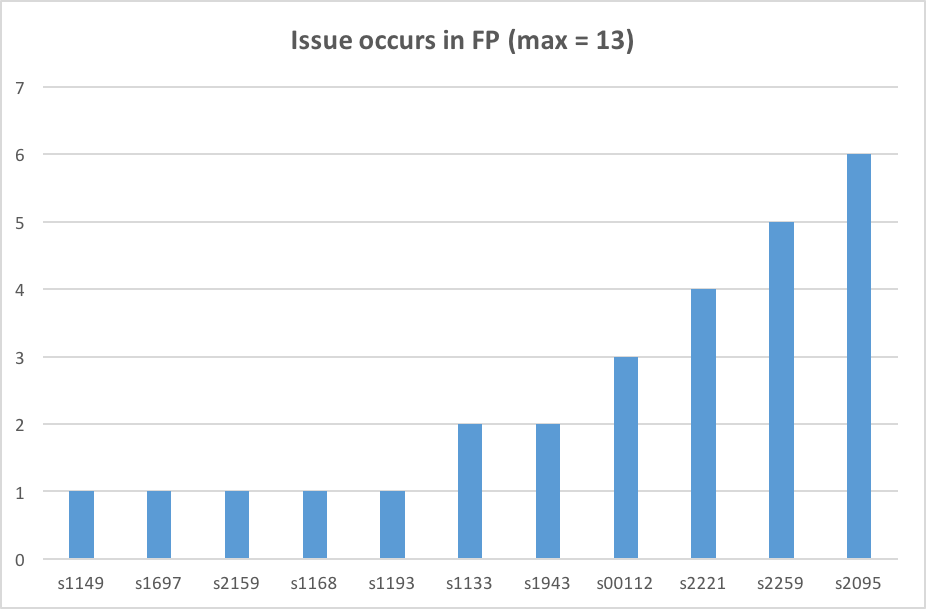
\includegraphics[width=0.7\textwidth]{figures/SQIssuesInFP.png}
	\caption{Number of times a SonarQube rule detected a bug for each of the FP cases}
	\label{fig:SQRulesForFP}
\end{figure}

\begin{table}[]
	\centering
	
	\label{table:SQrules}
	\begin{tabular}{lp{10cm}}
		\textbf{Rule} & \textbf{Description}                       \\ \hline
		s1149         & Failure to specify a locale when calling the methods toLowerCase() or toUpperCase() on String objects means the system default encoding will be used, possibly creating problems with international characters.                                                                                                                                                    \\ \hline
		s1697         & When either the equality operator in a null test or the logical operator that follows it is reversed, the code has the appearance of safely null-testing the object before dereferencing it. Unfortunately the effect is just the opposite - the object is null-tested and then dereferenced only if it is null, leading to a guaranteed null pointer dereference. \\ \hline
		s2159         & Comparisons of dissimilar types will always return false. The comparison and all its dependent code can simply be removed.                                                                                                                                                                                                                                         \\ \hline
		s1168         & Returning null instead of an actual array or collection forces callers of the method to explicitly test for nullity, making them more complex and less readable.                                                                                                                                                                                                   \\ \hline
		s1193         & Multiple catch blocks of the appropriate type should be used instead of catching a general exception, and then testing on the type                                                                                                                                                                                                                                 \\ \hline
		s1133         & This rule is meant to be used as a way to track code which is marked as being deprecated. Deprecated code should eventually be removed.                                                                                                                                                                                                                            \\ \hline
		s1943         & Using classes and methods that rely on the default system encoding can result in code that works fine in its "home" environment. But that code may break for customers who use different encodings in ways that are extremely difficult to diagnose and nearly, if not completely, impossible to reproduce when it's time to fix them.                             \\ \hline
		s00112        & Do not throw general Exception.                                                                                                                                                                                                                                                                                                                                    \\ \hline
		s2221         & Exception should not be caught when not required by called methods.                                                                                                                                                                                                                                                                                                \\ \hline
		s2259         & A reference to null should never be dereferenced/accessed. Doing so will cause a NullPointerException to be thrown.                                                                                                                                                                                                                                                \\ \hline
		s2095         & Java's garbage collection cannot be relied on to clean up everything. Specifically, connections, streams, files and other classes that implement the Closeable interface or it's super-interface, AutoCloseable, must be manually closed after creation.                                                                                                           \\ \hline
	\end{tabular}
	\caption{A selection of the SonarQube rules used during analysis}
\end{table}

For each rule we checked in how many cases it produced an issue. Figure \ref{fig:SQissuesForAll} shows these results. What becomes apparent is that there are a number of rules which almost always produce an issue, e.g. s1943 produces an issue in 112 of 115 cases. Note that s1943 is the rule that appeared in all three TPs. There are also rules that produce no results at all. For the set of selected rules, some only check test code. Of these, 6 out of 7 produce no issue in any case. The rule that did produce issues (in 12 cases) has the following text: ``\emph{When either the equality operator in a null test or the logical operator that follows it is reversed, the code has the appearance of safely null-testing the object before dereferencing it. Unfortunately the effect is just the opposite - the object is null-tested and then dereferenced only if it is null, leading to a guaranteed null pointer dereference.}'' \todo{more text baby!}

\begin{figure}[!ht]
	\centering
	\includegraphics[width=1\textwidth]{figures/SQIssuesForAllCases.png}
	\caption{Number of cases in which a SonarQube rule produces an issue}
	\label{fig:SQIssuesForAll}
\end{figure}

\section{Discussion}
There are a number of reasons why it is hard to measure whether SSCATs can actually find TBs. TBs are hard to generalize; coming up with a simple code example showcasing the test bug is hard. SSCATs only have rules to find very basic bug patterns in test code. All these patterns are insufficient to capture TBs. This statement however exposes one of the weaknesses of the analysis described in this chapter. The rules being used are selected based on expert opinion. It might happen that not every relevant rule is selected, or a rule is falsely mapped to a TB category. To mitigate these risks, selected rules were reviewed by another researcher at SIG. He also browsed the rules set of SonarQube to selectively test if no relevant rules were missed. All True Positives are again checked by another senior researcher to validate they were really True Positives.  

The SonarQube rule (s1943) that could find TBs also showed up in almost any investigated case, meaning at least one issue for the source code was generated. This reduces the usefulness of this rule, i.e. if it appears almost always, the change developers will ignore it becomes higher. However, we argue that when this rule detects an issue in test code, and a test fails, the developer should address it to prevent TBs of the OS category. 

The issues that appeared in the difference (in the FP cases) are mostly general issues. Some arise due to multiple Patches for a single TB. We analyzed the commit just before the first Patch, and the commit that provided the final Patch. If more than one commit was required to fix the TB, there could be many commits in-between, introducing or fixing bugs.

The results also showed that many SonarQube rules did not produce an issue in any case, that is; for all investigated TBs, no issue was generated by that rule. We looked into the analysis of SonarQube and asked the developers of SonarQube how the analysis works for some cases. If SonarQube does not have the binaries from a library, it cannot resolve method invocations, and even fails to detect unit tests in some cases. For instance, the rule that detects if an unit test contains a \texttt{Thread.toSleep()} method is a simple pattern match on $toSleep$ inside an unit test. However, since we statically tested all systems (without the binaries of the dependencies), SonarQube could not determine what methods were unit tests, and therefore did not produce any issues. 

Additionally, SonarQube stops with call-resolving when it encounters a method it cannot resolve. Consider the method \texttt{assertEquals(Thread.toSleep())} inside method \texttt{test()}. SonarQube encounters a method invocation it cannot resolve (\texttt{assert(..)} and does not look any further inside this method. As a result, \texttt{Thread.toSleep()} will not be resolved, while this method \emph{could} be statically resolved.  

Manually, we found some cases \todo{which?!} (JCR- and JCR-) for which throwing a general exception made the test fail.

\section{Conclusion}
\textbf{RQ3.1: What test bugs, as described by \Atestbugs{} can popular Java bug finding tools find?}  \\ 

In line with the findings of \Atestbugs{} we found only a very small fraction of TBs (2.3\%) could be found by SonarQube. All of these belonged to the Resource category, and the OS subcategory. We also found that SonarQube is ill-equipped to find issues in test code, when binaries are not available. \\ \\
\textbf{RQ3.2: To what extent can static source code analysis techniques be used to find test bugs?} \\

SonarQube requires the binaries of the testing framework to assess unit tests. Since we hardly found any TBs using SonarQube, we can argue that source code analysis without binaries is insufficient to find TBs. However, detecting unit tests without binaries is possible (see Chapter \ref{ch:TS}). The data we obtained in our study is insufficient to claim that static source code analysis without compiled code is insufficient to find TBs.




\chapter{Detecting Test Smells using Static Source Code Analysis}
\todo{Magiel: 'bad' tautologisch: refactor dit indien mogelijk}
We have shown in Chapter \ref{ch:SQ} that SonarQube is ill-equipped for finding Test Bugs (only 2.3\%!). Either the detection for certain bugs is completely absent or inadequate. This begs the question: How can we find or prevent test bugs from occurring? Closely related to the concept of test bugs, are test smells. A test smell is an indication of bad test code, similar to code smells being an indication of bad code in general. Intuition tells that when a developer writes bad code, there is a larger chance of introducing errors. To the best of our knowledge, there exist no research that has yet proven (or dis-proven) the relation between test smells and test bugs. 

In order to assess the impact of test smells on test bugs, we need to measure test smells in code that contained a TB. \Atestbugs{} gathered test bugs data for many Apache open source projects \cite{vahabzadeh2015empirical}. Working with this dataset comes with some challenges to overcome. Many open source systems are difficult to build, especially older versions. They require different versions of the JDK and JVM. Since snapshots are assessed, problems with missing dependencies become apparent. The correct jars are often not available online anymore. This is one of the reasons we chose to measure test smells using static analysis. This way we only need the source code. In section \ref{sec:TS_discussion} we discuss the impact static analysis has on the results. In short; the detected test smells are more indicators of poorly written test code. This is not that bad, for the goal of our research is to show if any relation between test smells and test bugs exists at all. 

Since there is relative little attention given to test smells, tools to detect these smells are sparse, and often of an academic nature. \cite{van2006characterizing, bavota2012empirical, greiler2013automated}. We implemented several test smells similar to \AsigTS \cite{van2006characterizing}. 

\AsigTS{} also defined weights for each test smell they measured. However, they only defined two test smells, where we measure five test smells. We also defined scores for each test smell, which are described in Section \ref{sec:eager} - \ref{sec:ctl}. We found that some test smells are far more severe as others, which has to be encompassed in relating one measure to another. One test method could for instance contain three assert methods without message (Assertion Roulette, see Section \ref{sec:AssertionRoulette}), while the other contains 20 asserts without messages. Clearly the latter is worse than the former.

\section{Background}
\todo{Where to put these list of concepts?}

\begin{itemize}
	\item Fixture
	\item Dynamic dispatch?
	\item Polymorphism?
\end{itemize}

The term \emph{Test Smell}; symptoms of poorly designed test code, was first introduced by \AtestSmell{}  \cite{van2001refactoring}. They proposed and explained 11 test smells. This set was expanded upon by \AtestxUnit{}, in his book about testing frameworks: \emph{xUnit Test Patterns} \cite{meszaros2007xunit}. \AtestFixture{} expanded the catalogue of test smells, introducing a number of novel ways to measure \emph{fixture} related smells \cite{greiler2013automated}. Informally, a \emph{test fixture} is a set of method calls and procedures to setup the SUT. \AsigTS{} defined two test smells based on the unit-coupling formalization framework introduced by \Aframework{} \cite{van2006characterizing, briand1999unified}. \Aframework{} describe their contribution as:  \emph{``Based on a standardized terminology and formalism, we have provided a framework for the comparison, evaluation, and definition of coupling measures in object-oriented systems.''}

\subsection{Formalization framework for the definition of coupling measures in object-oriented systems}
Trivial definitions for methods and classes are omitted. We assume that the reader is familiar with object-oriented concepts. Figure \ref{fig:ssOverview} presents an overview of a software system, and includes terms used in the definitions presented in this chapter.

\subsubsection{Class}
All classes for which $c$ is a superclass belong to the set of $Descendants$ of $c$.

\begin{definition}
	$Descendants(c) \subset C$ is the set of descendant classes of $c$
\end{definition}

\subsubsection{Method}
To define the set of methods in a software system, we simply define a set union over all methods in every class of the system.


	\begin{definition}[$M(C)$ - The set of all Methods] $M(C)$ is the set of all methods in the system and is represented as $M(C) = \bigcup\limits_{c \in C} M(c)$, \\
		
	where $M(c)$ is the set of methods for class $c \in C$.
	\cite{briand1999unified}
	\end{definition}

Methods can have different types, e.g. inherited, overriding, neither of the previous two. The set of implemented methods $M_i$ of a class $c$ is then defined as all the methods in $c$ that it inherits, but overwrites, or nonvirtual, noninherited methods. A method that can be inherited, overwritten, and for which dynamic dispatch is facilitated is called a virtual method. 

\begin{definition}
	$M_I(c) \subseteq M(c)$ is the set of implemented and overwritten methods, and the set of nonvirtual, noninherited methods of class $c$.
\end{definition}

\subsubsection{Method Invocation}
A method invocation occurs when one method calls another method. Invocations can be static and dynamic, where the difference is the time when a method invocation can be resolved. For static method invocations, the called method is determined by looking at the type of the identifier. Static method invocations are method invocations that can be resolved by looking at the type of the identifier, before runtime. Dynamic method invocations can only be resolved at runtime. Calling an abstract method through dynamic dispatch is an example of a dynamically invoked method. 

\begin{definition}[$SIM(m)$ - The Set of Statically Invoked Methods of $m$] \hspace{1em} \\
	Let $c \in C, m \in M_I(c)$, and $m' \in M(C)$. Then $m' \in SIM(m) \Leftrightarrow \exists_d \in C : m' \in M(d)$ and the body of $m$ has a method invocation where $m'$ is invoked for an object of static type class $d$.
\end{definition}


\todo{Explanation of def 3.1.5!}

\begin{definition}[$NSI(m_1, m_2)$ - The number of static invocation of $m_2$ by $m_1$] \hspace{1em} \\
	Let $c \in C, m \in M_I(c),$ and $m_2 \in SIM(m).$ $NSI(m_1, m_2)$ is the number of method invocations in $m_1$ where $m_2$ is invoked for an object of static type class $d$ and $m_2 \in M(d)$.
\end{definition}

\subsubsection{Example}
In code snippet \ref{code:formalizationExample} we provide example classes, methods and attributes, such that the reader can familiarize him/herself with the concepts defined by \Aframework, and presented in this chapter. The example is written in Java, which is an object-oriented language. For each of the defined concepts, the values are given, according to the framework. When appropriate, explanations are provided.

\begin{itemize}
	\item $C$: set of all classes = $\{Example, Node, InnerNode, Leaf\}$
	\item $M(C)$: set of all methods = $\{Node, InnerNode, Leaf, getIdentifier, children, childrenSum, invokeMethods\}$. Note that the first three methods are constructors.
	\item  $Descendants(Node)$ = $\{InnerNode, Leaf\}$. Note that if $InnerNode$ would be extended by $BinaryInnerNode$ and $UnaryInnerNode$, these would be added to the set of descendants of $Node$.
	\item $M_I(Leaf) = \{Leaf, children\}$. $M_I(Node) = \{Node, getIdentifier\}$.
	\item $SIM(Example) = \{InnerNode, Leaf, childrenSum\}$ 
	
\end{itemize}
\clearpage
\lstinputlisting[language=Java, caption=Object-oriented code example, label=code:formalizationExample]{CodeExample.java}
\clearpage

\subsection{Extending the coupling-formalization framework for test smells}

\AsigTS{} proposed a formalization framework to describe test smells, which also allows expressing the severity of test smells \cite{van2006characterizing}. There framework extends the formalization framework of Brand et al.,  Figure \ref{fig:ssOverview} defines several parts of a software system. A software system is composed of system code ($C$) and a number of libraries ($L$), which contain the libraries of the testing framework being used. The system code $C$ consists of production code $PROD$ and test code $TEST$. Both consist of a set of classes. $TEST$ consists of test helper classes, which are used by test methods. Test methods do the actual testing of the software system. The distinction between $PROD$ and $TEST$ is usually also practical, i.e. test classes are not included in the binaries when a software system is released. 
\begin{figure}[!ht]	
	\centering
	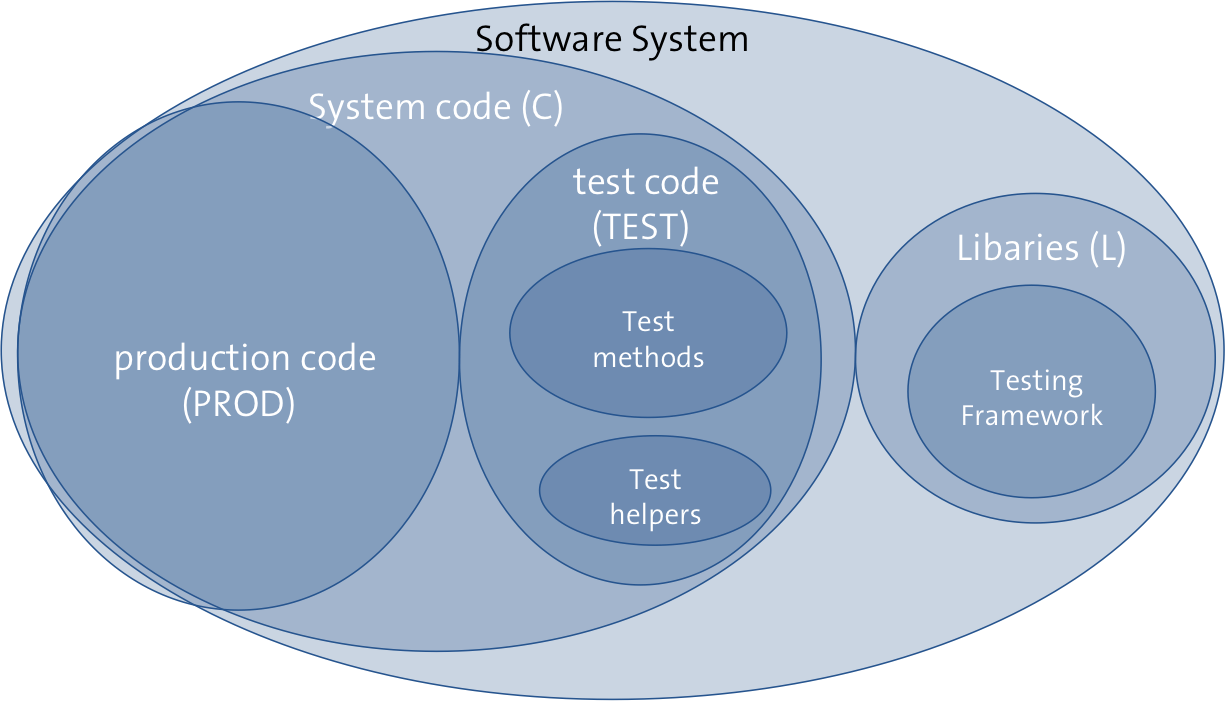
\includegraphics[width=0.8\textwidth]{figures/SoftwareSystemOverview.png}
	\caption{High level definitions of a software system, reproduced from \cite{van2006characterizing}}
	\label{fig:ssOverview}
\end{figure}

\begin{table}[]
	\centering
	
	\label{table:complexityTS}
	\begin{tabular}{|l|p{10cm}|}
		\hline 
		\textbf{Symbol}                           & \textbf{Entity}                                                                                                              \\
		\hline 
		$M(C)$                  & the set of all methods in the system \\
		$A(C)$ & the set of all attributes in the system      \\
		
		$M_i(c)$             & the set of methods implemented in $c$                          \\
		$Descendants(c)$       & the set of descendent classes of class $c$  \\
		
		$SIM(m) $ & the set of statically invoked methods of method $m$ \\
		
		$NSI(m_1, m_2)$ & the number of static method invocations of $m_2$ by $m_1$\\
		
		$AR(m)$ & the set of attributes referenced by $m$\\
		
		$M_{pub}(c)$ & the set of public methods of class $c$\\
		
		$uses(c,d)$ & A class $c$ uses a class $d$ if a method implemented in class $c$ references a method or an attribute implemented in class $d$ \\
		\hline
	\end{tabular}
	\caption{Definitions from Brand et al. \cite{briand1999unified}}
\end{table}

Usually, testing involves checking a result of exercising the SUT against an expected result. The testing framework provides methods to perform these checks, e.g. \texttt{assertTrue(), assertEquals(), assertNull()}.

\begin{definition}[Test Framework Check Methods - $TFCM$]
	\label{def:tfcm}
	$TFCM \subseteq M(UTFM)$, where $M(UTFM)$ is the set of methods the test framework offers.
\end{definition}

A test case is a class in the system that contains methods to test some behavior of the system. Usually, a test case groups methods that check the same part of the system. A test case extends the base test class of the test framework. 

\begin{definition}[Test Case - $TC$] 
	\label{def:tc}
	The set of test cases $TC$ = $Descendants(gtc) \subseteq C$, where $Descendants(gtc)$ is the set of classes that extend $gtc$, being the base test class used in the test framework. 
\end{definition}

A test helper class encapsulates commonly used functionality for testing in any of the testing phases (setup, stimulate, verify, teardown). Mock objects are an example of test helper classes. A class $c$ belongs to $TH$ if any of the methods of a class in $TC$ calls a method in $c$.

\begin{definition}[Test Helper - $TH$]
	
	Let $IM(c)$ = $\{IM(m) | m \in M(c) \}$, then
	
	$TH$ = $\{c \in C | MI(TC) \cap M(c) \neq \emptyset\}$
\end{definition}

Production code does not have a strict definition, for it merely is the remainder of the classes after we defined test code. Test code is simply the union of all test cases and test helper classes. 

\begin{definition}[Test Code - $TEST$ and Production Code - $PROD$] \hspace{1em}
	\label{def:TESTandPROD} 
	\begin{itemize}
		\item $TEST$ = $TC \cup TH$
		\item $PROD$ = $C \setminus TEST$
	\end{itemize}
	
\end{definition}

Unit tests are defined as public methods, having no parameters or return type, e.g. \texttt{void} return type in Java. The complete set of unit test, defined as $UT$ can be obtained by gathering all methods in $TC$ that satisfy all three conditions described above.

\begin{definition}[Unit Test - $UT$] \hspace{1em} \\
	\label{def:unitTest}
	$UT = \bigcup_{tc \in TC} \bigcup_{m \in M(tc)} : m \in \{M_{par0}(tc) \cap M_{pub}(tc) \cap M_{typ}(tc)\}$, where
	\begin{itemize}
		\item $M_{par0}(c) =$ the set of parameterless method of class $c$
		\item $M_{pub}(c) = $ the set of public method of class $c$
		\item $M_{typ}(c) = $ the set of methods without return type of class $c$
	\end{itemize}
\end{definition} 

An unit test usually consists out of four phases. First the system is $setup$ such that it is configured correctly, and all necessary resources to run the system are available. Secondly, the SUT is $stimulated$, meaning that the part of interest is called/run. The results of this phase are checked against expected values in the $verify$ phase. Finally, the system and resources are reverted to their original state, such that subsequent unit tests can run independently. This phase is called $teardown$.

\begin{definition}[Unit Test Phases] 
	\label{def:testPhases}
	An unit test consists of four phases; $setup$, $stimulate$, $verify$, $teardown$.
\end{definition}

For test smell detection we distinguish the types of method invocations an unit test can make. If an unit test calls a method in $TH$ or $TC$, that method invocation belongs to $IM_T$, i,e. the set of method invocations to test code. Similarly, we define $IM_P$ as the set of method invocations where the invoked method resides in production code. Finally, the set of invoked check methods $IM_C$ is defined.

\begin{definition}[Types of IM for unit tests] \hspace{1em}
	\begin{itemize}
		\item $IM_T(ut) = \{m \in IM(ut) | m \in M(TEST)\}$
		\item $IM_P(ut) = \{m \in IM(ut) | m \in M(PROD)\}$
		\item $IM_C = \{m \in IM(ut) | m \in TFCM\}$
	\end{itemize}
\end{definition}

\subsection{Test Smells}
We present for a number of test smells a short description as how they are described in literature. The following test smells are described by \AtestSmell \cite{van2001refactoring}.

The \emph{Eager Test} smell occurs when an unit test verifies too much functionality of the production code. An unit test is deemed eager if it verifies more than one production code method.

A \emph{Lazy Test} is the counterpart of an Eager Test, for it verifies too little functionality. An unit test is considered lazy when at least two unit tests verify the same production code method.

An unit test can have asserts that have no message, which make it harder for developers to debug tests. An unit test having at least two asserts, of which one contains no message is an \emph{Assertion Roulette} test.

Tests that verify the SUT using a \texttt{toString} method are prone to fail when the implementation of the \texttt{toString} method changes. A \emph{Sensitive Equality} test contains at least one assert invoking a \texttt{toString} method.

\emph{Conditional Test Logic} describes tests containing complexity structures (if, for while, try-catch, ...). Ideally, an unit test should be free of conditional logic to guarantee repeatable test results. If a test has at least two execution paths, the test might be unrepeatable. \AtestxUnit{} described several \emph{Conditional Test Logic} smells, see Table \ref{table:complexityTS} for an overview. 

\section{Tool architecture}
\toolName{} is build on top of the Software Analysis Toolkit (SAT), developed by SIG\footnote{\url{www.sig.eu}}. The SAT measures code based on static source code analysis, e.g. without the need for compiled or running code. The SAT mainly measures maintainability, and is build upon ISO 9126, which defines software quality into 6 subcategories, of which one is maintainability \cite{heitlager2007practical}. The ISO 9126 standard defines metrics which can be used to measure maintainability, giving a frame of reference to define a standardized framework. Since this paper, the SAT has been improved considerably, but the essence has remained the same: measure the maintainability of source code. 

The SAT measures source code, computes several metrics (LOC, duplication, usage-relations), which are then stored in a graph. \toolName{} queries this graph to compute metrics, which are than used to assess whether unit tests contain a particular test smell. For each detector, we describe what facts it measures, and when these facts result in a test smell. 

\toolName{} reports for every test smell the affected methods with their weight in a csv file. Descriptive statistics (average, percentiles, min, max, etc) for each smell, of the entire system are outputted to another csv file, using the Apache Commons Math3 \texttt{stats} library \footnote{\url{http://commons.apache.org/proper/commons-math/apidocs/index.html}}. Finally, \toolName computes frequency statistics for a given class, in particular cumulative percentages for each smell per method. Section \ref{sec:relateStats} describes how these measurements are used to answer the research questions.  

\toolName computes test smells in a number of steps, illustrated in Figure \ref{fig:toolSteps}. \todo{Make figure and} 

\section{Tool implementation}

\subsection{Obtain Test Code, Test Cases and Unit Tests}
\todo{Maybe change title of subsection?}
We obtain the set of Test Cases $TC$ by selecting all classes for which the class name matches one of the following regular expressions: "(.*)Test(.*)" or "Test(.*)". We assume that the common naming convention of the JUnit testing framework is followed, i.e. test class either starts with \emph{Test} or ends with \emph{Test}. Naturally, slight variations can occurs, e.g. ending on \emph{Tests}, which we also catch. We do not check if a class extends a base class of the testing framework, for this is already implied by the naming convention. \todo{say something about accuracy/precission/recall...}

According to Definition \ref{def:TESTandPROD}, test code, comprised of classes, consists of $TC$, and all classes that either access (invoke) methods or use attributes of a class in $TC$. The SAT produces a graph that has no information regarding attributes, so we only check on method invocations. Production code is simply the set of classes obtained by the set difference on the total set of classes and test code.

We obtain the set of unit tests by checking if a method has the \texttt{@Test} annotation, or the method name starts with $test$. These are conventions used when implementing the JUnit testing framework \todo{ref mayhaps?!}. Additionally, we only consider the stimulate and verify phases in our analysis, see Definition \ref{def:testPhases}. Sometimes, developers encapsulate verification in one or multiple custom verification methods. In that case, the unit test does not call any JUnit assert methods, but defers this to helper methods. Only measuring the unit test in that case will give false results. See Code example \ref{Code:deferredComplexity}, where unit test \texttt{test()} asserts the correctness of an object by calling \texttt{assertTableNotNull(Table t)}. The McCabe of \texttt{test()} is 1, but executing this silly test can lead to different results depending on the day! We should therefore also count the complexity of \texttt{assertTableNotNull(Table t)}. In this example, we define the McCabe complexity of \texttt{test()} as 2.

\begin{lstlisting}[language=java, caption=Complexity example of unit test with custom verification method., label=Code_deferredComplexity]
@Test
public void test() {
	// setup 
	setupResources();
	
	// stimulate
	Table t = new Table();
	t.initTable();
	
	//verify
	assertTableNotNull(Table t);
	
	//teardown
	cleanupResources();
}

public void assertTableNotNull(Table t) {
	Day day = CalendarUtils.getDay();
	if (day.isSunday()) {
		thrown new Exception(e) {
			System.out.println("We do not test on sundays!");
		}
	} else {
		assertNotNull("table should be properly initialized!", table);
	}	
} 
\end{lstlisting}

\subsubsection{Custom Verification Method-Linking problem}
Linking custom verification methods to the correct unit test is a non-trivial task for real-world software systems. Developers can create chains of test helper methods, deferring the actual JUnit assert call. Developers might also create custom test frameworks, with Abstract classes holding the verification methods, and Concrete classes the unit tests, i.e. the complete unit tests, as defined above might be scattered in multiple classes and packages. 

We can solve the Custom Verification Method-Linking problem by call-graph analysis. A call-graph is a directed graph of method calls, where $n_1$ calling $n_2$ is expressed as an edge going from node $n_1$ to $n_2$. The SAT does static call-graph analysis, which is explained in the next section.

\subsection{SAT call resolving for Java}
We rely on the SAT call-resolving for measuring a number of test smells, being eager test, lazy test, indirect testing, and for testers only. Call-resolving maps method calls made inside a method to the called methods based on name, if there is a unique mapping possible. See figure \ref{fig:call_resolving} for some scenarios. On the left we have a test method containing three method calls. Method call \texttt{c()} can easily be resolved on name, for it occurs only once in the system (in \texttt{org.company.data.B}).

Method call \texttt{a()} occurs in both classes \texttt{A} and \texttt{B}. We first look at the parameters, removing any calls from the set of candidates if their parameter list differs. In this case no such eliminations can be made. Since Java is a statically typed language, we can also look at the imports, and match on package name. This resolves the call to method \texttt{a()}. 

Finally, we have to resolve the call to method \texttt{b()}. In this case we cannot match on package name, for both candidates are in the same package. We check for the type of the identifier (\texttt{id}) invoking \texttt{b()}. Sometimes, the type of the identifier can only be determined at runtime, e.g. if it occurs in a conditional statement. In these cases, the SAT does not resolve the call and flags it as \emph{ambiguous}. Calls to methods that cannot be found in the source code are flagged as \emph{unresolved}.

\begin{figure}[!ht]
	
	\centering
	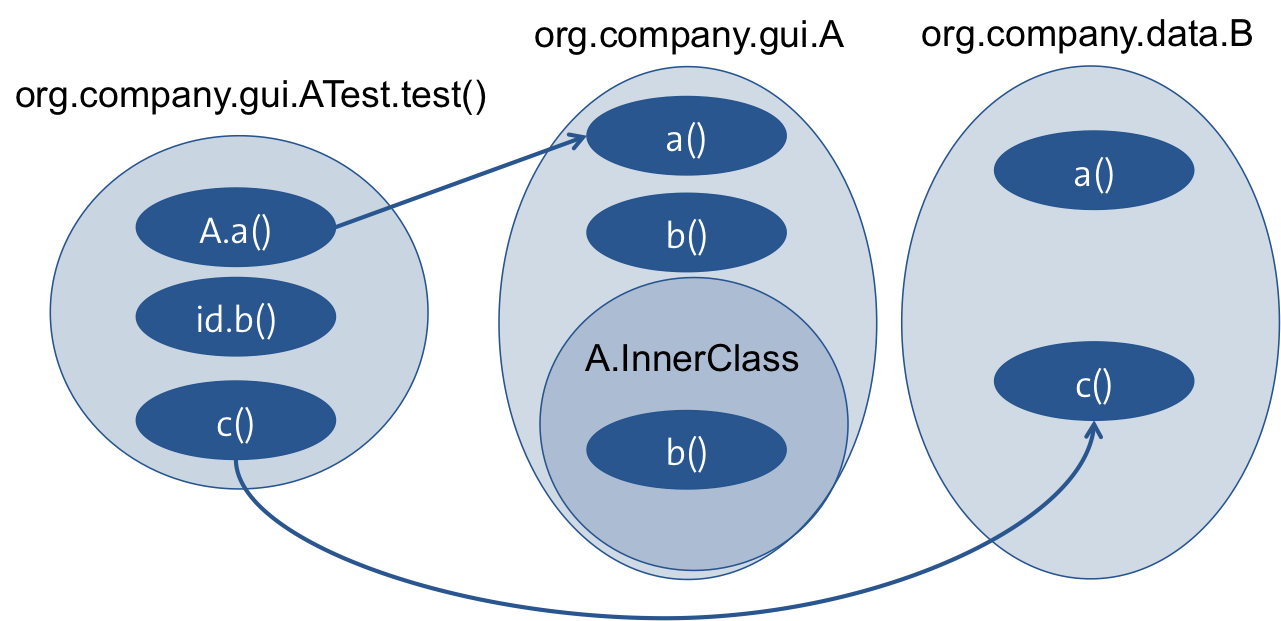
\includegraphics[width=0.7\textwidth]{figures/call_resolving.png}
	\caption{Call-resolving scenarios for Java}
	\label{fig:call_resolving}
\end{figure}

\subsection{Solving the Custom Verification Method-Linking problem}
\label{utClojure}
To promote reuse and automated testing, developers encapsulate verification logic in separate check methods. Starting from an unit test, there can be a chain of methods leading up to the method that actually does the verification, i.e. contains a method in $TFCM$, see Definition \ref{def:tfcm}. If we want to measure an unit test, we should include all methods that are relevant for a given unit test. Therefore we define the so-called $Clojure(ut)$. This is all the direct and indirect method invocations starting from an unit test, ending in a method containing a method invocation to a method in $TFCM$. We stop when reaching a method in production code. 



\subsection{Eager Test}
\label{sec:eager}
\emph{Unit test invoking more than one production method.}\\

An eager test verifies too much functionality in a single test method \cite{meszaros2007xunit}. There are a multitude of issues with an eager test being: hard to read, hard to maintain, hard to localize errors, and coding errors might slip in when writing the test logic. The latter two can be mapped to obsolete TBs (\ref{sec:obsoleteTB}) and semantic TBs (\ref{sec:semanticTB}), since an eager test makes it harder to see the mismatch between test code and production code. \AsigTS{} also mention the numerous stimulate-verify cycli in eager tests \cite{van2006characterizing}. This results in dependencies between cycli within a unit test, possibly making the test flaky when one cycle relies on a previous cycle that did not respond in time.

\subsubsection{Formal definition}
Use Section \ref{sec:utClojure}
\begin{definition}[Number of production method uses]
	content...
\end{definition}

\begin{definition}[Eager Test]
	\begin{itemize}
		\item 
	\end{itemize}
\end{definition}

Our analysis for eager tests considers test phases; implicit setup, stimulate and verify. Implicit setup is done within an unit test. Since we cannot distinguish setup code from stimulate code, we simply consider method invocations from the entire unit test. 

To statically determine if a test is eager, we look at the \emph{usages} of this unit test. An unit test contains the Eager Test smell if it uses two or more production units. We exclude any calls to third-party code, since we are only interested in the SUT. Furthermore, we exclude constructor calls, since these will most likely not be the tested methods.  

\subsubsection{Ranking}
We can rank eager tests based on their \emph{weight}, defined as the  number of usage relations with unique production methods. An unit test $t1$ that uses more unique production methods as $t2$ is considered worse. Intuitively, a developer would have to consider more code when $t1$ fails, as compared to $t2$.

\subsubsection{Example}
 In Figure \ref{fig:EagerTest} eager test $testB$ uses both $a()$ and $b()$, and has weight 2. 



Our analysis for eager tests considers test phases; implicit setup, stimulate and verify. Implicit setup is done within an unit test. Since we cannot distinguish setup code from stimulate code, we simply consider method invocations from the entire unit test. 



\begin{figure}[!ht]
	
	\centering
	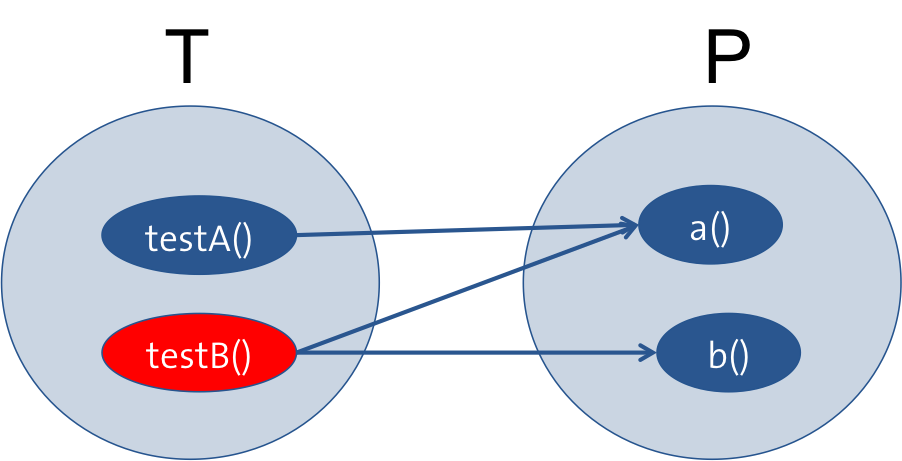
\includegraphics[width=0.5\textwidth]{figures/EagerTest.png}
	\caption{In red an Eager Test}
	\label{fig:EagerTest}
\end{figure}

\subsection{Lazy Test}
\label{sec:lazy}
\emph{Two or more unit tests having identical method invocations.}\\

The Lazy Test smell occurs when one production method is being tested by multiple test methods. Ideally, tests should be self-contained and fully test a single production method. When the production method changes, both tests need to be examined to see if changes are necessary. This again introduces the risk for Obsolete TBs.

Unit tests in a group ($n > 1$) testing the same production method, all having the same fixture, are considered lazy tests \cite{van2001refactoring, meszaros2007xunit}.\\

Since we only have information on usage relation between methods, we cannot infer what the tested method is. So we look at all method invocations inside an unit test (both to production and test code). When we find a pair of tests having an identical set of usage relations, we group them together. In Figure \ref{fig:LazyTest} tests $testA$ and $testB$ both use $\{a,fixture\}$, so considered lazy, whereas $testC$ only uses $a$. The reason $testC$ is not in this set is because its fixture differs from $testA$ and $testB$. 

Our analysis for lazy tests considers the same phases as Eager Tests, see \ref{sec:eager}

To order lazy tests on severity, we look at the number of tests having the same usage set. A larger number means that more tests are testing the same production method. A change in the tested method requires the developer to look at many tests, introducing a window to make mistakes.

\begin{figure}[!ht]	
	\centering
	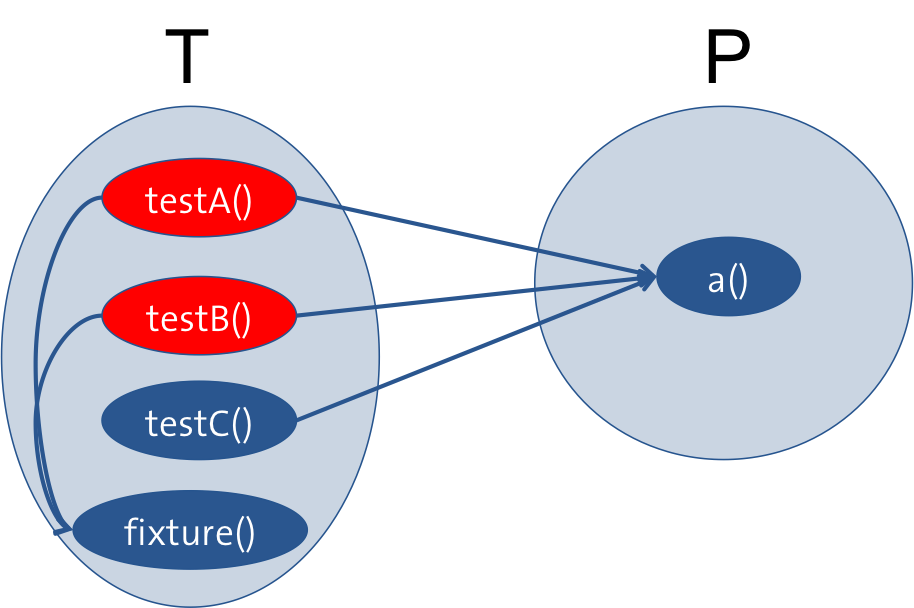
\includegraphics[width=0.5\textwidth]{figures/LazyTest.png}
	\caption{In red two lazy tests}
	\label{fig:LazyTest}
\end{figure}

\subsection{Sensitive Equality}
\emph{unit test with at least one assert that contains a \texttt{toString} call} \\

The Sensitive Equality test smell occurs when asserting values that are prone to change based on implementation. An example of this is relying on the \texttt{toString()} method for equality. If the implementation of this method changes, the check does not hold anymore.\textsl{}

\subsection{Assertion Roulette}
\label{sec:AssertionRoulette}
\emph{unit test contains at least two assertions, and at least one of these assertions has no message}. \\

\todo{Story inconsistent}
When an unit test fails, it stops at that point, i.e. assertions after the point of failure are not checked. When an unit test contains numerous assertions without error messages, it becomes very hard to determine what the cause of failure was. Consider a test with the Assertion Roulette smell in code example \ref{Code_Assertion_Roulette}. Eclipse for instance reports that on line 9 there is an assertion failure, where \texttt{true} was expected, but \texttt{false} was encountered. The developer than has to determine the call-trace leading to the failure. In this case the statement on line 4 made the second assert fail.

\begin{lstlisting}[language=java, caption=Code with assertion roulette smell, label=Code_Assertion_Roulette]
@Test
public void test() {
	checkValue(2);
	checkValue(1);
	checkValue(6);
}

private boolean checkValue(int value) {
	assertTrue(value > 1);
	assertNotNull("value shouldnt be null!",  value);
	assertEquals(2, value);
}
\end{lstlisting}

This definition of an assertion roulette smell we provide differs slightly from the definition given by van Deursen \cite{van2001refactoring}. They defined an Assertion Roulette test when it had two assertions, one without a message. When a developer investigates a test with two asserts, one having no message, he can see what assert failed based on the occurrence of an error message. Onwards of three asserts this is not possible anymore. 

To statically detect assertion roulette smells, we rely on the implementation of the testing framework. There exist numerous testing frameworks, each defining different assert methods and different ways to add failure messages to an assert. In real world software systems, testing frameworks are used to make life easier for developers. Some of these are JWalk, TestNG, JUnit, Mockito and Powermock. \footnote{\url{https://blog.idrsolutions.com/2015/02/8-useful-java-testing-tools-frameworks-programmers-developers-coders/}}

Our detection of the Assertion Roulette smell relies on pattern matching, making the support of many testing frameworks time-consuming. Therefore, we chose to focus on the JUnit testing framework, for it is commonly used in ASF projects, which are the subject of analysis. \todo{how many plusminus?}

To determine the number of arguments in an assert, we wrote a simple parser that takes as input the method invocation (assert method with parameters), and recursively determines the number of parameters. This is done by recursively reducing the input parameters, such that nested method calls, strings, array object creation and escaping characters are eliminated. What remains is the top level parameter. 

A custom written solution is applied over usage of an existing parser for several reasons. First, we eliminate the overhead of a parser solution, for we only require the number of parameters from an assert method. Secondly, the custom parsing solution is completely context-independent, i.e. any input can be correctly parsed. Code of the parameter reduction algorithm can be found in Appendix \ref{ap:functionParamsAlgo}. Limitations are extensibility with respect to supporting more testing frameworks. Some test frameworks for instance use the builder pattern \todo{ref} to string together a number of verification methods. The current implementation of the parameter discovery algorithm cannot cope with this.

\subsection{Conditional Test Logic}
\label{sec:ctl}
\emph{Unit test having a McCabe value larger than one.} \\

Ideally, unit tests should have zero complexity, i.e. always following the same path. Whenever flow structure elements are introduced in test cases (if, else, while, for, etc) tests become progressively harder to understand, maintain, and debug when they fail. Meszaros described several categories of conditional test logic smells \cite{meszaros2007xunit}. Table \ref{table:complexityTS} shows an overview. A number of them we can measure by simply measuring the McCabe complexity, i.e. number of execution paths. The McCabe complexity measure provides an easy way to calculate complexity structures in test code, but has its limitations. The measure is without semantical meaning, so Flexible Tests can not be measured. We can also not distinguish between the other test smells (complex teardown, production logic in test, conditional verification logic, multiple test conditions). 

We must also exclude try-catch blocks, for these are often used for Exception testing. If we take a threshold value of 3, we automatically exclude pure Exception tests (a try-catch block has a McCabe value of 2). However, having a higher threshold will result in False Negatives, i.e. missed conditional test logic smells. Therefore we rely on pattern matching, to find try-catch blocks in an unit test. If such a block exists, we reduce the complexity by one, i.e. disregarding the try-catch construction, for it is likely to be an exception test. The test case can of course contain other complexity structures, so we do not disregard the entire test if we encounter a try-catch block.

There are numerous different ways to write unit tests \cite{meszaros2007xunit}. One of which is to encapsulate verification logic into a separate method. We have to distinguish systems that use this type of testing. Consider method $testA$ calling method $checkResultsA$, which does the verification. The complexity of $testA$ is calculated as $McCabe(testA) + McCabe(checkResultsA)$. \todo{ref naar beschrijving hoe deze te onderscheiden!}

\begin{table}[]
	\centering
	\begin{tabular}{|l|p{10cm}|}
		\hline 
		\textbf{Type}                           & \textbf{Description}                                                                                                              \\
		\hline 
		Flexible Test                  & The test code verifies different functionality depending on where or when it is run. (e.g. using \texttt\{System.time\}) \\
		Conditional Verification Logic & Tester tries to prevent execution of assertions when SUT fails to return right objects, or assert collections etc.       \\
		Production Logic In Test       & Conditional verification logic in test.                                                                                  \\
		Complex Teardown               & Teardown of persistent data structures may leave these data structures in an unexpected state.                           \\
		Multiple Test Conditions       & Test tries to apply same test logic to many sets of input values, each with its own corresponding expected result.  \\
		\hline    
	\end{tabular}
	\label{table:complexityTS}
		\caption{Complexity Smells
			 \cite{meszaros2007xunit}}
\end{table}
\chapter{Are Test Smells an Indication of Test Bugs?}
\label{ch:TS}
We have shown in Chapter \ref{ch:SQ} that SonarQube is not capable of finding Test Bugs. Either the detection for certain bugs is completely absent or inadequate. This begs the questions: How can we find or prevent test bugs from occurring? Closely related to the concept of test bugs, are test smells. A test smell is an indication of bad test code, similar to code smells being an indication to bad code in general. Intuition tells that when a developer writes bad code, there is a larger chance of introducing errors. To the best of our knowledge, there exist no research that has yet proven (or dis-proven) the relation between test smells and test bugs. 

We will investigate if such a relation exists in real world software systems, by answering the following questions: \\
\\
\textbf{RQ4.1: Does bad test code indicate test bugs?} \\

We will answer this question by looking at the test smells occurring in the code affected by the test bug. We want to see if there are significantly more, or worse test smells as compared to``bug free'' parts of the system.\\ \\
\textbf{RQ4.2: Do Test smells predict the occurrence of test bugs?} \\

For each test smell we can measure its severity. Do test bugs occur in parts of the system that have test smells of high severity? Are there healthy parts of the system that  also contain test smells of high severity?

This chapter is structured as follows: in Section \ref{sec:TS_measure} we show how we measure the different test smells, and explain the tool we build. In Section \ref{sec:TS_relate} we show the experiment design; how we selected the systems, dataset, and how and what we measured. Section \ref{sec:TS_results} shows the results. In Section \ref{sec:TS_discussion} we discuss implications of the findings and talk about threats to validity. Section \ref{sec:TS_conclusion} draws conclusions.


\section{Measuring the relation between Test Smells and Test Bugs}
\label{sec:TS_relate}

Our goal is to show if there exists a relation between Test Smells and Test Bugs. For one, we need a system with actual test bugs. Secondly, we need a tool to detect test smells in this system. Thirdly, we need a measure to indicate how one relates to the other.

There are a number of approaches we can take, each differing in level of detail. We can employ the same approach as in Chapter \ref{ch:can_tools_find_TBs}. We would measure the affected code by the Patch, noting down the test smells before and after the fix. A simple comparison would indicate whether the fix reduced the number or severity of the measured test smells. While a good approach to validate bug-finding rules, this approach is too detailed for the often broad definition of a test smell. Most test bug fixes are small, sometimes just one line of code, so the impact on test smells is minimal.

If we take an evolutionary point of view we can look at test smells as eroding the test code, i.e. making it more susceptible for test bugs. Intuitively, bad test code will more often lead to test bugs, compared to good test code. To show if this relation actually exists in real software systems, the following steps are taken:

\begin{enumerate}
	\item Checkout the system just before the test bug fix.
	\item Measure test smells in the system.
	\item Compare the code regions causing the test bug with the average quality of the test code (measured in terms of test smells).
\end{enumerate}

\subsection{Compare }

\section{Results}
\label{sec:TS_results}

\section{Discussion}
\label{sec:TS_discussion}

Note: unresolved calls are not bad, since we only want to assess the code itself, e.g. test methods generally only test the production code, so we do not care about dependencies etc.

\section{Conclusion}
\label{sec:TS_conclusion}

\chapter{Discussion}
Should this be a self-contained chapter?

\chapter{Conclusion}
summary of conclusion in chapter 2, and add conclusion of chapter 3. Draw conclusions from both performed studies.


\chapter{Literature Study}
\todo{Refactor into thesis, what parts to exclude??}

\section{Test Code Quality and Its Relation to Issue Handling Performance}

\AtestCodeQuality{} studied the relation between test code quality and issue handling performance \cite{athanasiou2014test}. They constructed a quality framework for test code on three categories:

\begin{enumerate}
	\item \textit{completeness}: how complete is the system tested? Achieved using program slicing to statically estimate code coverage. Also the decision point coverage is estimated.
	\item \textit{effectiveness}: hoe effective is the test code in detecting and localization faults. 
	\item \textit{maintainability}: how maintainable is the test code. They build a  maintainability model, which is based on the maintainability model of SIG. 
\end{enumerate}

The test quality model was calibrated using benchmarking. They tested the quality model on two commercial software systems. The results were validated by two experienced consultants who knew a lot about the system. The results were closely alligned, but the consultants generally rated the test code quality of a system higher.

To measure the relation between test code quality and issue resolution speed, a study was conducted on several open source projects. \AtestCodeQuality{} found that test code quality has a significant correlation with productivity and throughput. Productivity was measured as the normalized number of resolved issues per month divided by the number of developers. Throughput was measured as the normalized number of resolved issues per month divided by the KLOC. 

Issue resolution speed; time between assignment of issue to a developer, and resolving the issue, showed no significant correlation with test code quality. Issue resolution time is hard to measure due to several confounding factors:

\begin{itemize}
	\item Hard to measure number of developers working on an issue. One developer can be assigned, but multiple work on the issue.
	\item A developer might not work constantly on the same issue.
	\item Issues get reopened, which adds resolution time. Issues not yet being reopened might not accurately reflect resolution time.
	\item The experience of the developer is not taken into consideration.
\end{itemize}




\section{Concept-Based Failure Clustering}
DiGiuseppe et al. \cite{digiuseppe2012concept} proposed a novel way to cluster program failures based on semantics. The stack trace responsible for the failure is compared based on the occurrence of words, e.g. in variables and comments. Their paper is a proof of concept, and shows for a medium sized system that semantic based clustering produces less clusters as control-flow based clustering while maintaining the same accuracy. 

Issue reports contain a lot of semantic information. This paper showed that it can be promising to incorporate this information into a classification model for test bugs, based on clustering. 


\section{Empirically Detecting False Test Alarms Using Association Rules}

Herzig et al. \cite{herzig2015empirically} tried to reduce the number of false alarms in test bugs during integration testing. They used associate learning to classify issues about test bugs being false positives. Accuracy was about 85-90\% with the number of correctly detected false positives at the end ranged from 34 to 48\%. They mainly investigated integration tests on two Windows systems for a period between one and two years. 

Integration tests consist of a number of test steps. When one test step fails the integration test fails. The integration test is not immediately aborted, but continues to run resulting in an array of failed or passed test steps. These arrays where used as antecedents (left hand side of association rule) and linked to either a false positive or an actual production code bug. If a rule occurs enough, is non-contradictory, and has high confidence (the rule predicts a given outcome with high accuracy), the rule is kept. 

For \textit{Windows 8.1} the maximum net gain (in man hours) was 1.7 hours per day. For \textit{Dynamics XS} it was 14 minutes per day. In a real world company one still needs to investigate each case, since there exist cases where a bug is introduced into the system but classified as False Positive. 

\section{An Empirical Analysis of Flaky Tests}
Flaky tests are tests that sometimes fail due to concurrency issues \cite{luo2014empirical}. \Aflaky{} started from commit messages and sampled 201 commit messages (previously identified as fixing a flaky test). For each of these commits they determined the root cause of the flaky test, how it manifests itself in the code, and how it was fixed. The top three categories of flaky tests are:
\begin{enumerate}
	\item \texttt{async wait} (45\%): A test makes an asynchronous call and does not wait properly for the resources to become available. Almost all flaky tests (96\%) fail independent of the platform. Roughly a third uses a simple method call with time delays to enforce ordering. 85\% involve only one ordering and do not wait for external resources. This means that flaky tests in this category could be detected by inserting one time delay in a certain part of the code without the need to control the external environment. Using \texttt{waitFor} (often instead of \texttt{sleep}) causes 54\% of bugs to be fixed. 
	\item \texttt{concurrency} (20\%): caused by different threads interacting in a non-desirable way, but not in the \texttt{asynch wait} category. Almost all bugs in this category involve two threads or can be reduced to two threads. 97\% fails due to concurrent accesses on memory objects only. Concurrency bugs are solved in a number of ways; adding locks, making the program deterministic or changing conditions. 
	\item \texttt{test order dependency} (12\%): The outcome of a test depends on the order in which tests are executed. The problem may arise when two tests depend on a common resource, which is not properly managed. About half (47\%) are caused by a dependency on external resources. By cleaning the shared state between test runs proved successful in solving the bug in 74\% of the cases. 
\end{enumerate}
Other causes of flaky tests are fixed in a variety of ways. When a fix is made in the code under test (CUT), most fixes (96\%) also fix a bug in the CUT.

\Aflaky{} provide patterns for detecting flaky tests, which can be incorporated into a test bug detection tool. The patterns are based on static source code analysis.


\section{Finding Bugs is Easy}
There exist many tools that find bugs with extensive analysis and complicated algorithms. \AFB{} found some cases were production code contained trivial bugs, easily detectable by a bug pattern. On this bases they developed FindBugs, a static analysis tool for Java Bytecode \cite{hovemeyer2004finding}. 

FindBugs works on the basis of a bug pattern. A bug pattern is a part of source code that usually contains a bug. They illustrated several patterns, their rationale, and showed evidence of the occurrence of these patterns in real world software systems. FindBugs is designed to be easily extended by plug-ins. 

The aim of FindBugs is not to be as accurate as possible, or have a high recall. It is designed to be easily incorporated into the development process, and find relatively simple bugs. \AFB{} showed, for a number of bug patterns, that FindBugs has an acceptable false positive rate.

\Atestbugs{} listed a number of test bug categories, which can be translated into FindBugs bug patterns. 

\section{Experiences Using Static Analysis to Find Bugs}

FindBugs, a popular static analysis tool for Java Bytecode is analyzed regarding its usage in real world settings. \AFBEval{} explain their experience with developing and deploying FindBugs \cite{ayewah2008using}. FindBugs was introduced in 2004 \cite{hovemeyer2004finding}.

\AFBEval{} deployed their tool at Google. They found that FindBugs usage is dependent on formal policies. Without, it is up to the developer how FindBugs is used, and usage may very wildly. 

They also found that developers review a high percentage (around 90 \%) of high risk warnings. Lower level warnings are reviewed as well, but are context-specific. Developers fix warnings ad-hoc, can use annotations to suppress warnings, or use filtering techniques to filter out uninteresting warnings or false positives. There are a number of strategies to keep track of FindBugs warnings, and keep them relevant. Companies can use store warnings in a database, collect and send warnings after each day via email, immediately fix warnings or incorporate warnings in their review policies.

\AFBEval{} also discuss the limitations of FindBugs, which is useful when considering building new detectors, i.e. for test bugs.

\section{A Comparison of Bug Finding Tools for Java}
\AComparisonBugTools{} studied several bug finding tools for Java, and compared their results \cite{rutar2004comparison}. FindBugs is a static analysis bug finder that processes Java Bytecode and is based on syntax and dataflow analysis. JLint is similar to FindBugs, but \textit{``also includes an inter-procedural, inter-file component to find deadlocks by building a lock graph and ensuring that there are never any cycles int he graph''}. FindBugs' dataflow analysis is restricted to the method level. PMD performs syntactic checks on source code, and is more focused on detecting violations in stylistic conventions. Bandera is a verification tool based on model checking. The programmer can use annotations to include specifications to be checked. Without annotations, Bandera primarily checks for standard synchronization properties. ESC/Java is based on theorem proving and performs formal verification of properties of Java source code. The programmer adds preconditions, postconditions and loop invariants in the form of annotations. Without annotations ESC/Java looks mainly for null pointer dereferences and array out-of-bounds errors. 

Interestingly, \AComparisonBugTools{} found no significant correlation among pairs of tools. They tested for a relation between code size (lines of code with spaces and comments removed) and number of reported warnings on the class level. They also tested if the number of reported bugs for one tool correlated with other tools. 

\AComparisonBugTools{} proposed a meta-tool that combines the results of different tools and ranks classes based on two metrics; normalized warning total and unique warning total. For the latter, they counted the same error messages as one, e.g. cascading error messages for JLint. For the former they counted all error messages a tool issues per class, added the result for all tools, and normalized the result by the maximum value of issued errors for that class. They found a significant correlation between the two metrics. When a class scored high in normalized warning total, it could score very low in unique warning total, and vice versa. The goal of these metrics was to give developers information on potentially interesting classes that individual tools would miss. \AComparisonBugTools{} found several examples where their meta-tool indicated a class to be important, but individual tools would have rated it much less important.

%This paper explains the technologies behind a number of popular Java bug finding tools. Reference point when extending research, e.g. step 3 in the timeline, see \ref{sec:timeline}


{%\tiny
\bibliographystyle{abbrv}
\bibliography{researchProposal}
}

\appendix

\chapter{Automation algorithm}
\todo{refactor}
\textbf{Steps}\\
\begin{enumerate}
	\item For every $ASFProject_i$ in $ASF_P$ \textbf{do}
	\item \hspace{1cm}For every sampled $ITB$ in $ASFProject_i$ \textbf{do}
	\item \hspace{2cm} \label{step_checkout_solvingCommit} Checkout commit identified by $ITB$ in seperate branch.
	\item \hspace{2cm} \label{step_prop_file} Add \texttt{sonar-project.properties} file to root directory.
	\item \hspace{2cm} \label{step_runSQ} Run test bug analysis by running \texttt{sonar-runner} in the root folder of the project.
	\item \hspace{2cm} \label{step_parent_commit} Checkout parent commit of commit identified in \ref{step_checkout_solvingCommit}
	\item \hspace{2cm} repeat steps \ref{step_prop_file} to  \ref{step_runSQ}.
	\item \hspace{2cm} \label{collectResults} Collect results
	\item \hspace{2cm} \label{step_comp_diff} Compute diff of results.
	\item \hspace{2cm} \label{step_cleanup} Cleanup resources.
	\item \hspace{1cm} \textbf{od}
	\item \textbf{od}

\end{enumerate}

\chapter{Test Smell Tool implementation}
\label{ap:code}
This chapter contains implementation details about certain parts of \toolName{'s} code.

\section{Determine the number of function parameters}
\label{ap:functionParamsAlgo}
\begin{lstlisting}[language=java, caption=Number of parameters algorithm, label=Code_parameterAlgorithm]

/*
	* returns the number of parameters in this function
*/
public static int functionParameters(String function) {
	ParsingUtils parsingUtils = new ParsingUtils();
	String fnStripped = StringUtils.stripTill('(', function);
	String fnStripped2 = fnStripped.substring(1);
	// find function with 0 parameters, i.e. f()
	if (parsingUtils.removeWhiteSpace(fnStripped).length() == 2) {
		return 0;
	}
	// find function with >= 1 parameters
	return parsingUtils.countFunctionParameters(fnStripped2);
}

/*
	* @pre: function is a string, starting from the arguments of a function, excluding the first parenthesis.
	* @pre: function has at least one parameter.
	* @post: the number of parameters of the original (top level) function.
*/
private int countFunctionParameters(String function) {
	// every function has at least one parameter (@pre)
	if (function.length() == 0) {
		return 1;
	} 
	char next = function.charAt(0);
	String newString = function.substring(1);
	switch(next) {
		case ',' : return 1 + countFunctionParameters(newString);
		case '(' : newString = removeUntil(')', newString); return 0 + countFunctionParameters(newString);
		case '"' : newString = removeUntil('"', newString); return 0 + countFunctionParameters(newString);
		case '\'' : newString = removeUntil('\'', newString); return 0 + countFunctionParameters(newString);
		case '{' : newString = removeUntil('}', newString); return 0 + countFunctionParameters(newString);
		default : return 0 + countFunctionParameters(newString);
	}
}

private String removeUntil(char c, String str) {
	if (str.equals("")) {
		return str;
	}
	String newString = str.substring(1);
	if (str.charAt(0) == c) {
		return newString;
	}

	switch (str.charAt(0)) {
		case '(' : return removeUntil(c, removeUntil(')', newString));
		case '"' : return removeUntil(c, removeUntil('"', newString));
		case '\'' : return removeUntil(c, removeUntil('\'', newString));
		case '{' : return removeUntil(c, removeUntil('}', newString));
		case ')' : return newString;
		case '}' : return newString;
		default : return removeUntil(c, newString);
	}
}

private String removeWhiteSpace(String str) {
	return str.replaceAll("\\s+","");
}

\end{lstlisting}
\end{document}
